\documentclass[a4paper]{ctexbook}

\usepackage{geometry}
\geometry{left=3cm,right=3cm,top=4.0cm,bottom=4.0cm}

\hfuzz=100.0pt   % TODO: 临时解决方案

\usepackage{graphicx}
\usepackage{subcaption}
\usepackage{amsmath} %equation
\usepackage{amssymb}

% \usepackage{mathabx} %rightrightharpoons
\newcommand{\rightrightharpoons}{{\Longrightarrow}}   % TODO: fix it



\newcommand{\exampledp}{\texttt{ExampleDP}}
\newcommand{\para}[1]{\smallskip\noindent {\bf #1}}

%Math macros
\newtheorem{definition}{定义}
\newtheorem{lemma}{引理}
\newtheorem{theorem}{定理}
\newtheorem{proof}{证明}
\newtheorem{corrollary}{推论}


\usepackage{hyperref}
\usepackage[backend=biber,style=gb7714-2015,gbpub=false,isbn=false,doi=false,gbtitlelink=true,url=false,sortlocale=zh__pinyin]{biblatex}
\addbibresource{../intro-cn/all-all.bib}

\begin{document}
 
%\tableofcontents
\chapter{cap 章节}

%SDN数据通路编程容量问题

%\section{摘要}
%
%高级编程和可编程数据通路是软件定义的网络(SDN)的两个关键能力。连接这两个能力的一个基本问题是,给定的高级SDN程序是否可以实现到给定的低级SDN数据通路上。考虑到所有可以在给定数据通路上实现的高级程序都可以看作是数据通路的编程能力,我们将此问题称为SDN数据通路编程容量问题(SDN Datapath Programming Capacity Problem)。本章中,我们基于一个通用的场景,即高级、数据面无关、算法性的SDN程序和目前最新的多流表流水线SDN数据通路,对软件定义网络数据通路编程容量问题进行研究。特别的,把数据面无关的SDN程序想作是``计算",把数据通路流水线想作是``计算能力",我们引入了一个全新的框架,叫做SDN特征函数(SDN Characterization Functions),以此将SDN程序与数据通路映射到一个统一的空间,并导出关于SDN数据通路编程能力的相关结果。最后,我们给出对相关结果的实验验证。


\section{引言}\label{sec:introduction}
%\cleet{Introduction placeholder text}
SDN的一个主要研究方向是可编程、高效的数据通路(例如, OpenFlow1.3~\cite{openflow1-3}, OF-DPA~\cite{OF-DPA}, P4~\cite{P4})。只有实现可编程性,SDN数据通路才能支持各种不断发展的应用场景。同时,数据通路必须高效,能够满足高吞吐量和高成本效益等要求。在过去的几年中,多流表流水线已经成为SDN数据通路的一个关键部分(例如, Domino~\cite{sivaraman2016packet}, Forwarding Metamorphosis~\cite{rmt})。


%A problem of efficient datapaths, however, is that they can be low level to program.

然而,高效数据通路的一个问题是,它们必须经常以低级语言(甚至配置)进行编程,导致开发低效。例如,TCAM对于实现高吞吐量至关重要,然而它不支持逻辑非。因此,SDN的第二个主要研究方向是数据通路无关的、高级编程,并通过抽象来隐藏底层数据通路细节。在过去几年中,也出现了多个高级SDN编程模型(例如, Frenetic~\cite{foster2011frenetic}, Maple~\cite{maple})。

随着这两个研究方向的发展,一个基本问题则是:给定的高级程序能否在给定的低级数据通路上实现。对这一问题的良好理解将有助于高级SDN程序的设计和数据通路的设计。给定一个固定的数据通路(例如,一个固定的流水线结构,OF-DPA),数据通路的供应商可以提供相关的高级程序的指南。反过来,给定一组高级程序,可以来设计支持这些程序的最紧凑的数据通路。即使对于可重新配置的数据通路(例如, P4),由于重新配置是昂贵且耗时的,因此可以基于对该问题的理解指导设计更健壮的数据通路。考虑到所有可以在给定可编程数据通路上实现的高级程序可以看作是数据通路的容量,我们将这一基本问题定义为SDN数据通路编程容量问题。

然而,解决数据通路容量问题并非易事。考虑一个简单的数据通路,Simple-DP。如图~\ref{cap:fig:fig1-update}所示,它是最简单的数据通路之一,由构成流水线的三个表组成,其中第一个表(\texttt{t1})在源IP上匹配,并且可以跳到以下两个表,这两个表都在目标IP上匹配。

\begin{figure}[h!]
    \centering
    \vspace{-0.1in}
    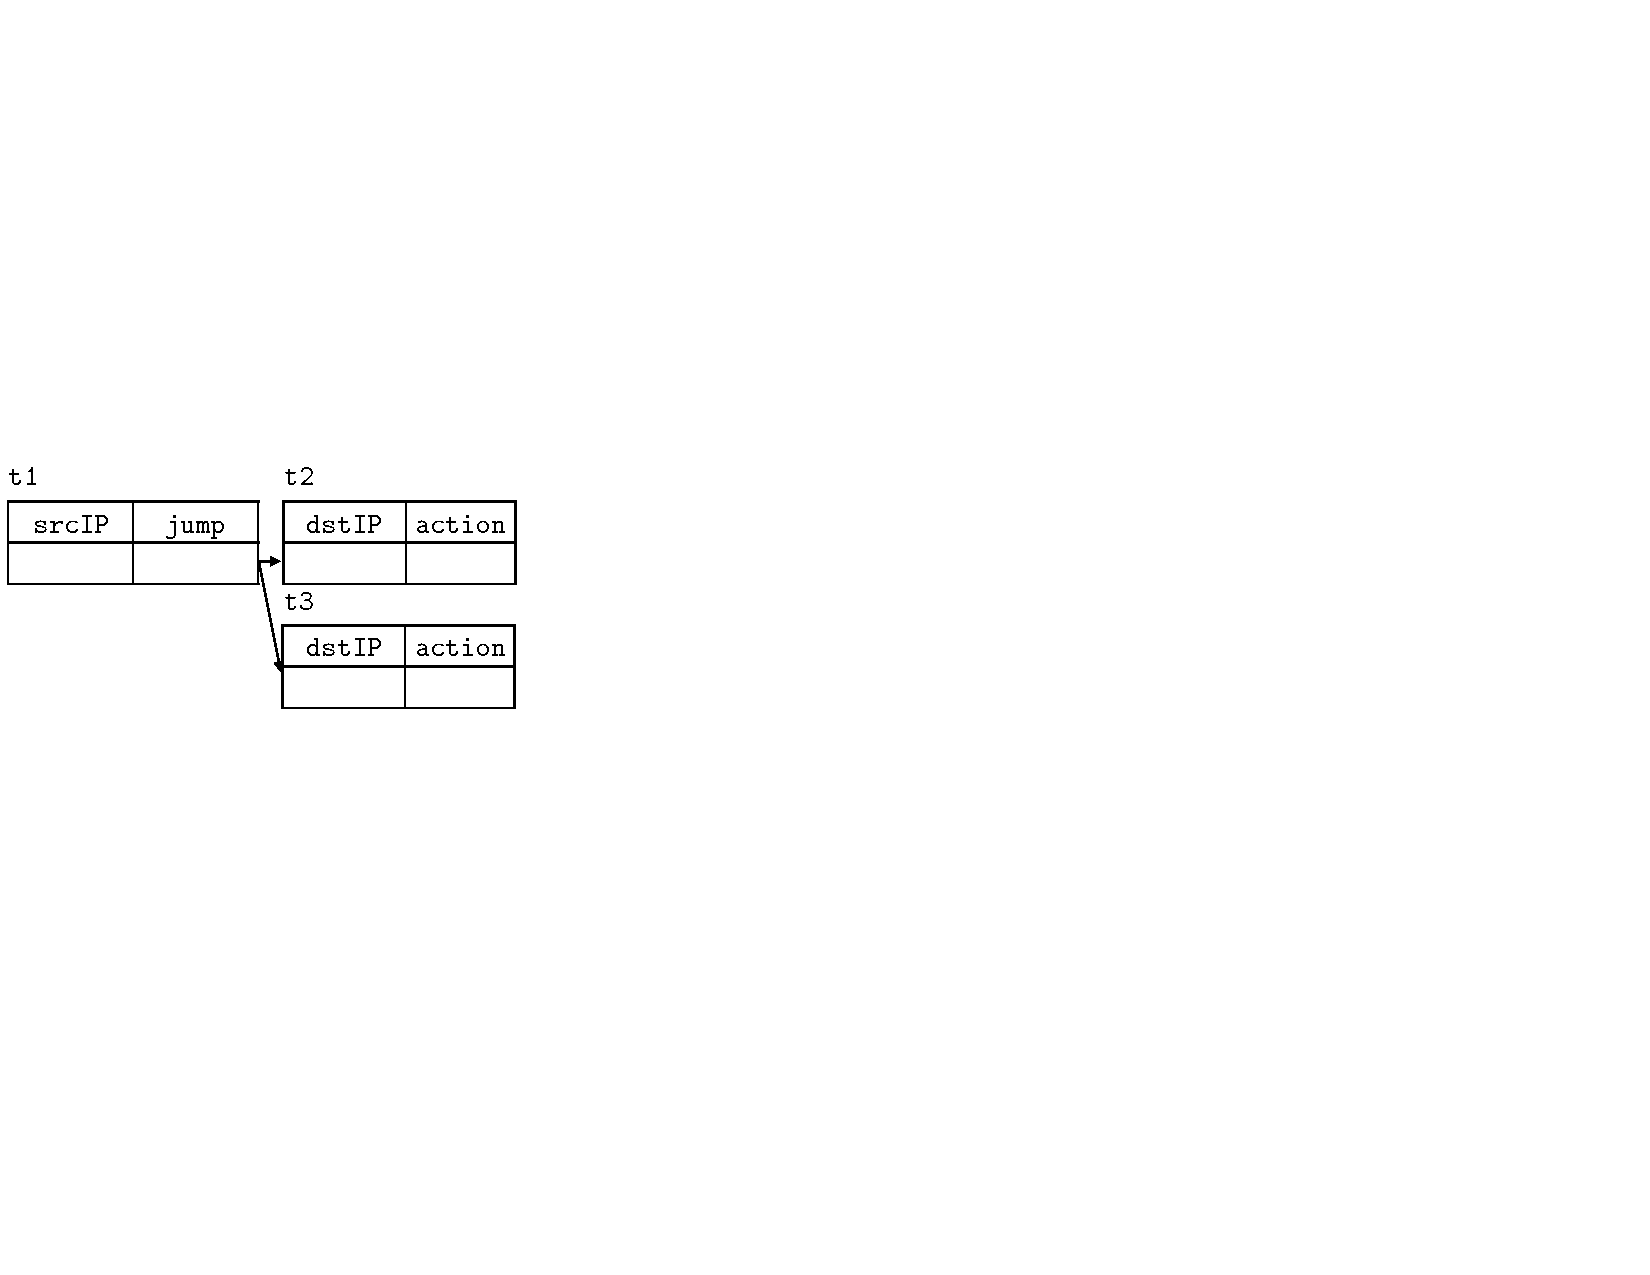
\includegraphics[scale = 0.7]{figures/figure1.pdf}
    \vspace{-0.1in}
    \caption{一个简单的数据通路示例: Simple-DP}
    \vspace{-0.1in}
    \label{cap:fig:fig1-update}
\end{figure}

我们再考虑下面两个简单的高级SDN程序,它们都采用算法性、事件驱动的编程模型(下面会给出有关编程模型的更多详细信息)。我们可以发现第一个程序可以通过Simple-DP实现,而第二个程序则不能。

{\small
    \begin{verbatim}
    //  Routing Function: secureL3Route
    L1: def secureL3Route(Addr srcIP, Addr dstIP):
    L2:   if srcIP == 10.0.0.1:
    L3:     return Forward(port=shortestPath(dstIP))
    L4:   else:
    L5:     return Drop();
    \end{verbatim}
}

{\small
    \begin{verbatim}
    //  Program: twoHostL3Route
    L1: def twoHostL3Route(Addr srcIP, Addr dstIP):
    L2:   if srcIP == 10.0.0.1:
    L3:     return Forward(port=shortestPath(dstIP)) 
    L4:   elif srcIP == 10.0.0.2:
    L5:     return Forward(port=securePath(dstIP))
    L6:   else:
    L7:     return Drop();
    \end{verbatim}
}

尽管前面的数据通路和高级程序是最简单的,但它们已经可以说明解决SDN数据通路容量问题并不明显。由于需要实现多个服务,一般数据通路和高级程序可能要复杂得多,因此它们在分析中可能会带来严峻的挑战。本章的目标是试图得到一个系统的方法来解决SDN数据通路容量问题。

本文的贡献可以概括如下。首先,我们提出了一个统一的特征函数空间来消除程序结构和流水线布局的复杂性和不一致性。其次,我们在这个函数空间中定义了一个比较运算,用来判断一个高级程序是否可以在给定的流水线上实现。

%本文的其余部分组织如下。我们在章节~\ref{sec:model-and-main-results}中给出了模型的精确定义。主要结果在章节.~\ref{sec:main-results}中给出。章节~\ref{sec:evaluation}是我们的测试评估结果。章节~\ref{sec:related-work}介绍相关工作。


\section{相关工作}\label{sec:related-work}
\para{高级SDN程序编译器}: 过去几年,人们提出多种允许程序员用高级语言编写SDN程序,并将这些程序编译成流表的系统。因为它们需要检查高级程序到交换机流表的转换,因此这些系统与本章工作相关。我们将这些系统分为两类:无层和分层。

无层系统(如SNAP~\cite{arashloo2016snap}, FML~\cite{hinrichs2009practical}, FlowLog~\cite{flowlog},  Maple~\cite{maple}),要求程序员通过编写数据包处理函数的形式,指定数据包的转发行为。然后SDN控制器使用这些函数来配置和更新网络状态。这样的系统启发了流水线容量定理中函数的概念。但是,这些系统在没有实际执行的情况下无法验证提交的函数是否可以写入给定的流水线结构。

分层系统如Frenetic家族(Frenetic~\cite{foster2011frenetic}, Pyretic~\cite{reich2013modular})提供了一个两层编程模型,其中控制器程序指定感兴趣的事件,然后在这些事件发生时通过计算新的网络策略来响应。同样,这样的系统无法验证给定控制器程序的输出是否可以写入交换机的流水线。

\para{流水线定制语言}:流水线定制语言(如P4~\cite{P4}, PISCES~\cite{shahbaz2016pisces}, Concurrent NetCore~\cite{schlesinger2014concurrent})和我们的流水线容量定理之间有一些相似之处,同样对流水线行为进行了分析以及保证。例如,Concurrent NetCore的类型系统确保用于部署到流水线的任何程序都具有某些属性~\cite{schlesinger2014concurrent},而PISCES的交换机规范允许编译器分析流水线并优化其性能~\cite{shahbaz2016pisces}。
然而保证流水线属性或提高性能与验证编译是否可行是不同的。


%\para{Multi-switch network programming:} Our pipeline capacity algebra is related to other systems that facilitate multi-switch network programming, specifically DIFANE~\cite{DIFANE} and TableVisor~\cite{TableVisor}. These systems, however, focus on distributing a centrally specified flow table/flow table pipeline across a given network, whilst our algebra verifies that generic high level language programs can be written to it.

\para{流水线设计}:流水线设计方案,如Jose等人~\cite{Jose-et-al}考虑的将数据包程序编译到可重构交换机、Sun等人~\cite{Sun-et-al}的软件定义流表流水线、FlowAdapter~\cite{pan2013flowadapter}和Domino~\cite{sivaraman2016packet}显然与我们的流水线容量定理相关,因为它们检查硬件约束下的流水线布局设计。然而,Jose等人,Sun等人,和FlowAdapter着重于将逻辑查找表或多流表流水线映射到物理表,而我们的流水线容量定理侧重于通用程序,而Domino考虑的是较弱的硬件约束条件(如有状态操作)。


\section{模型}
\label{sec:model-and-main-results}

我们首先给出高级SDN程序和低级数据通路的模型。由于SDN的主要关注点是路由,因此我们这里将高级SDN程序称为路由函数。由于多流表流水线是SDN数据通路的最先进技术,因此我们这里将流水线作为数据通路对象进行研究。

\subsection{路由函数模型}
\label{subsec:function-model}

\para{路由函数}:我们将一个路由函数表示为$f$。我们考虑它是一个逻辑上集中的、确定的函数,并用高级语言编写。SDN控制器对进入该控制器网络的每个数据包逻辑上执行该函数~\cite{maple},以计算出该数据包的全网范围的路由。

每个$f$在数据包上的执行要读取数据包的一组属性(称为匹配字段)$\mathcal{M} = \langle m_1, ..., m_n \rangle$ (例如, \texttt{<srcIP, dstIP, ...>})。我们用$M$表示数据包匹配字段在$\mathcal{M}$中的一个子集。此外,我们用$dom(M)$来标识一组匹配字段$M$的域。$f$的执行会从一组(对数据包的)有效操作$\mathcal{R}$返回一个路由操作,(例如, \texttt{Drop, Forward(port=2)}):

%Any subset of these match fields' $M \in \mathcal{M}$ value $v_i(M)$, however, is restricted to the domain of valid values $dom(M)$ specified by the match fields' headers' network protocols. Given this restriction, $f$ may be summarized as a mapping from values in $f$'s match fields' domain to actions in $\mathcal{R}$:

\begin{equation*}
f : dom(\mathcal{M}) \rightarrow \mathcal{R}.
\end{equation*}

这样的函数所在的空间标识为$\mathcal{F}$。

\para{示例}:我们用如下的路由函数\texttt{onPkt}来演示我们路由函数模型的一些关键特性。
\begin{verbatim}
\\  Routing function: onPkt
    Map hostTbl[key: dstIP, value: switch]
    Map condTbl[key: (dstIP, port), value: cond]
    Map routeTbl[key: (switch, cond), value: outPort]
L1: def onPkt(Type ethType, Addr srcIP, Port srcPort, \
          Addr dstIP, Port dstPort):
L2: if (ethType != IPv4):
L3:   return Drop()
L4: if (verify(srcPort, srcIP)):
L5:   dstCond = condTbl[dstIP, dstPort]
L6:   dstSw = hostTbl[dstIP]
L7:   return Forward(port = routeTbl[dstCond, dstSw])
L8: return Drop()
\end{verbatim}

具体来说, \texttt{onPkt}读取匹配字段
$\mathcal{M} = \langle \texttt{ethType}, \texttt{srcIP}, \texttt{srcPort}, \texttt{dstIP}, \texttt{dstPort} \rangle$ 
并将$\mathcal{M}$域中的每个值映射到$\mathcal{R}=\{\texttt{Drop()}, \texttt{Forward(port=x)} \}$中的路由操作。虽然我们将\texttt{onPkt}以命令式函数写出,需要强调的是我们的模型是完全通用的,并且没有指定编程范式。


具体地说,\texttt{onPkt}的前三行声明了键值表:\texttt{hostTable}和\texttt{condTable}。它们分别把每个IP地址和一个连接交换机以及主机条件(例如, 身份验证状态)进行关联,而\texttt{routeTable}将(交换机、条件)映射到其转发端口。在\texttt{onPkt}的主体部分上,\texttt{L2}和\texttt{L3}检测并丢弃非IPv4流量,而\texttt{L8}则丢弃来自未验证的终端的流量。如果验证通过,\texttt{L5}到\texttt{L7}设置\texttt{dstCond}和\texttt{dstSw}变量,然后基于这两个变量从\texttt{routeTbl}返回路由操作。



\para{路由函数数据流图}:由于一般的路由函数可以具有任意的、复杂的控制结构,我们将路由函数转换为数据流图(Dataflow Graph,DFG)以更好地表示其结构。我们把$f$的DFG表示为$G_f$。

具体来说,要计算$f$的$G_f$,我们必须删除$f$中所有的控制流依赖。这些依赖通过以下转换被删除:

\begin{itemize}
  \item 通过将$f$转换为静态单赋值形式(Static Single-Assignment, SSA)来移除赋值语句顺序依赖;
  \item 通过将分支的条件值赋给guard变量来移除分支,并将对这些guard的依赖性附加到\texttt{if}和\texttt{else}块中的所有语句;
  \item 通过将程序循环转换为黑盒函数来删除它们,黑盒函数的输入为循环中读取的所有变量,输出为循环中写入的所有变量。
\end{itemize}

例如,我们的示例路由函数\texttt{onPkt}转换如下:

\begin{verbatim}
L1: def onPkt(...):
L2: g0 = (ethType != IPv4)
L3: if  g0: return Drop()
L4: g1 = verify(srcPort, srcIP)):
L5: if  g1: dstCond = condTbl[dstIP, dstPort]
L6: if  g1: dstSw = hostTbl[dstIP]
L7: if  g1: return Forward(port = routeTbl[...])
L8: if !g1: return Drop()
\end{verbatim}

注意\texttt{onPkt}的\texttt{L2}处的\texttt{if}语句已经从条件表达式变成了guard变量 \texttt{g0},\texttt{g0}又被附加给了\texttt{L3},这一行之前是在\texttt{if}块内的。

在给出了这个转换后,我们定义$f$的$G_f$:

\begin{definition} 一个路由函数$f$的数据流图DFG $G_f = (V_f, E_f)$是一个从转换的$f$生成的点带权的有向无环图,其中:
\begin{itemize}
  \item $V_f$中的每个点$v_f$是$f$的一个变量;
  \item 一个$v_f$的权重是它的域值范围大小;
  \item 当两个变量之间存在一条$E_f$中的有向边时,意味着源变量出现在目的变量的赋值声明中。
\end{itemize}
\end{definition}

作为示例,我们给出 \texttt{onPkt}的DFG如下:
\begin{figure}[tbh]
    \centering
    \vspace{-1mm}
    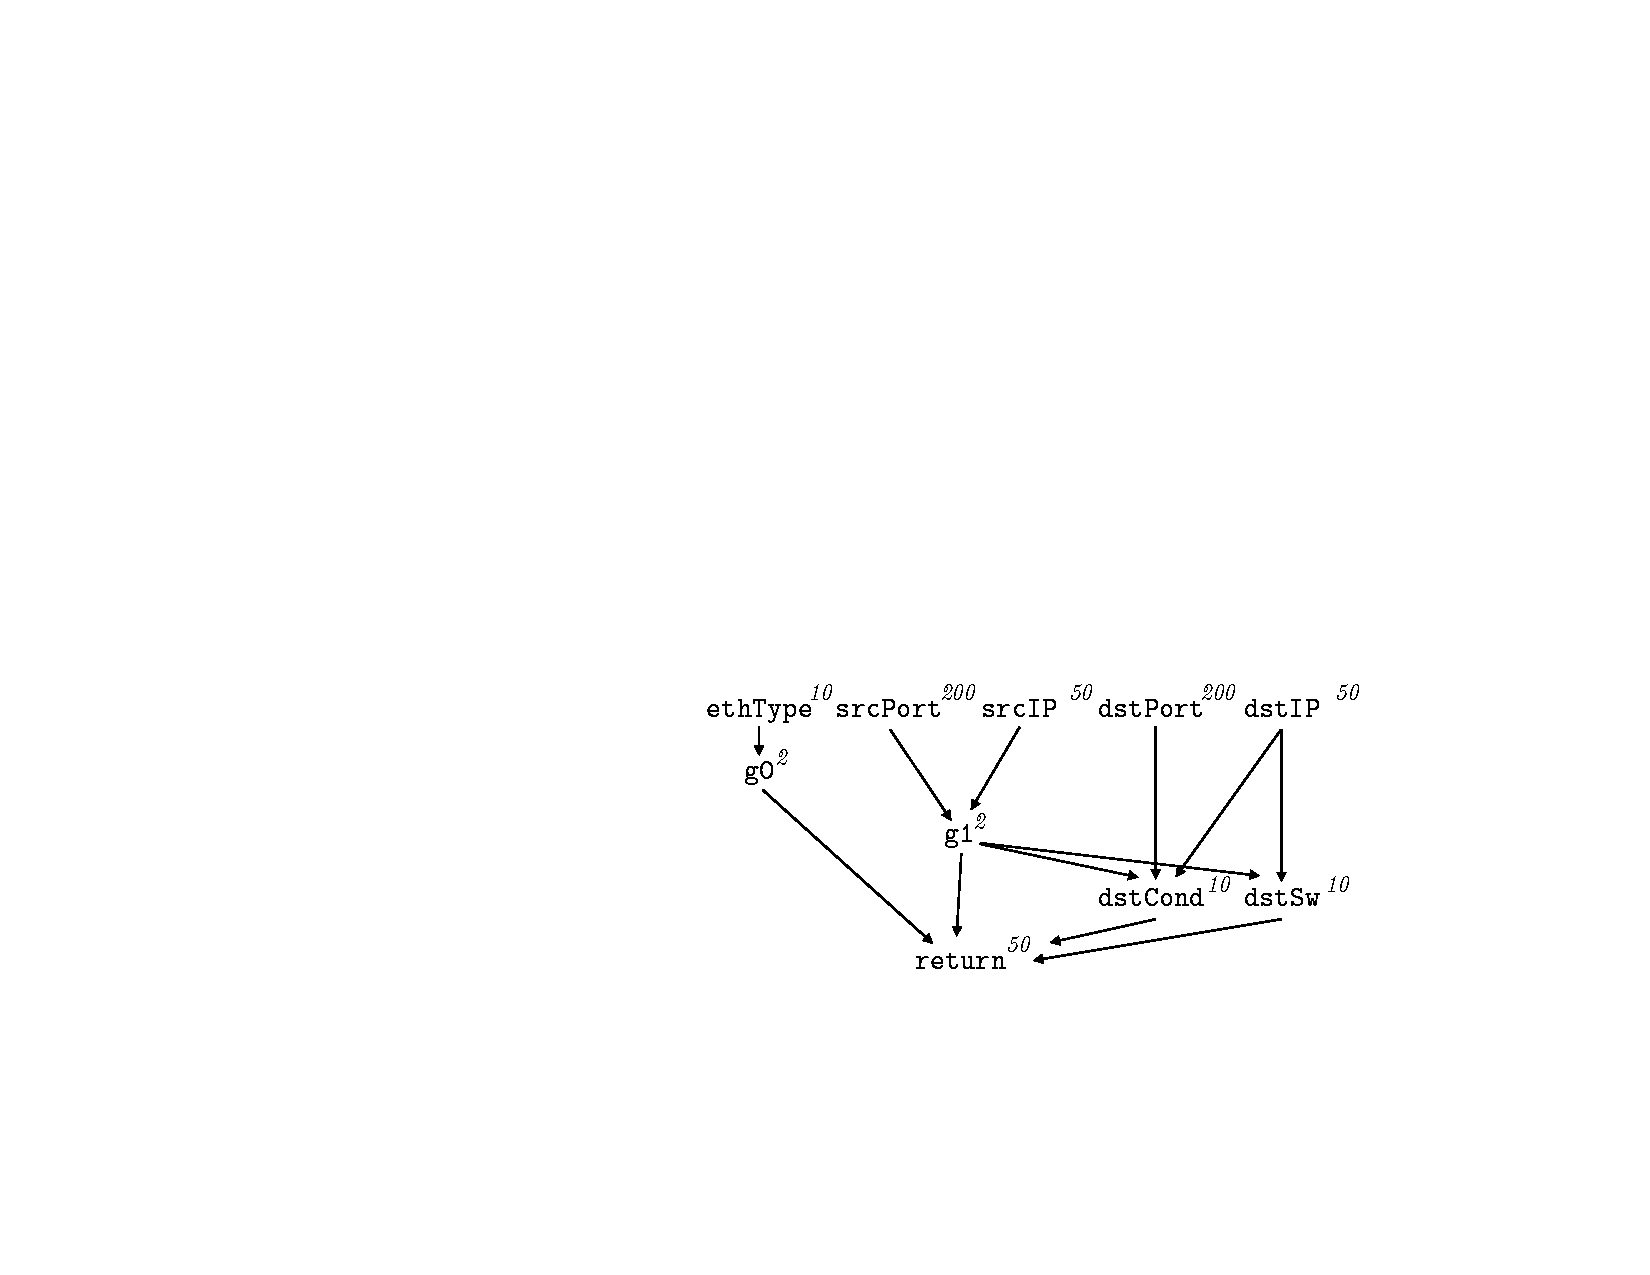
\includegraphics[scale = 0.6]{figures/figure2.pdf}
    \vspace{-2mm}
    \caption{路由函数\texttt{onPkt}的DFG $G_{\texttt{onPkt}}$}
    \label{cap:fig:onpkt-dfg}
    \vspace{-2mm}
\end{figure}

可以看到,点\texttt{dstSw}是由其赋值声明中的两个变量\texttt{g1}和\texttt{dstIP}派生得到的。该点的权重$10$表示\texttt{dstSw}的域值范围大小。


%IPv4 packets' destination endpoints are mapped to their attachment switch and host condition in \texttt{L4} and \texttt{L5}, which \texttt{L6} uses to look up the packet's next hop forwarding port.

%Elaborating, \texttt{onPkt}'s first three lines declare key-value map state variables. \texttt{hostTable} and \texttt{condTable} associate layer 3 endpoints with their attachment switch and host condition (\eg\ authentication status) respectively while \texttt{routeTable} maps switch condition pairs to their forwarding port. Moving on to \texttt{onPkt}'s body, \texttt{L1} and \texttt{L2} drop non-IPv4 traffic, while \texttt{L3} and \texttt{L7} drop traffic from unverified endpoints. Verified IPv4 packets' destination endpoints are mapped to their attachment switch and host condition in \texttt{L4} and \texttt{L5}, which \texttt{L6} uses to look up the packet's next hop forwarding port.


%\yry{An example function}

%An $f$ specifies such network behavior by conceptually running on every packet entering the network and returning a network routing action for each. We denote  the space of all network routing actions an $f$ can return $\mathcal{R}$, and the space of all $f$  $\mathcal{F}$.

%When a packet enters the network, $f$ reads its header's match fields  $\langle m_1, ..., m_n \rangle$. We denote the set $\forall$ packet match fields $f$ reads $\mathcal{M}$, and subsets of $\mathcal{M}$ $M_i$. Further, we say that the value of a subset of a given packet's header match fields $M_i$ is $v_i(M_i)$. These match fields values are restricted  to the domain of valid values specified by the match fields' header's network protocol, $dom(M_i)$. 

%Given the above, $f$'s type signature is:

\subsection{流水线模型}
\label{subsec:pipeline-model}

我们考虑目前最新的数据通路设计:多流表流水线架构。我们首先对一个流水线$pl$中的一个表$t$进行建模,然后给出对于流水线的清晰定义。

%A pipeline $p$ is a singly rooted dag (directed, acyclic graph) of tables $\{t_i\}$. 

\para{流水线中的表}: 每个流水线中的表$t \in pl$是精准匹配的match-action表。$t$的匹配操作可以是:(1)一个路由操作;(2)对$t$的输出寄存器$r(t)$的写操作以及对 $pl$中的后续表的跳操作;(3)对 $pl$中的后续表的简单跳操作。并不是所有的$t$都输出路由操作。我们把输出路由操作的$t$称为出口表。

每个$t$匹配着一组输入 $I(t)$。输入 $I(t)$包含数据包的匹配字段 $m_i \in \mathcal{M}$ 和前序表的输出寄存器$r(t)$。$t$的关键限制是它可以包含的最多规则数量和$r(t)$的比特位长度,在这里我们对应地表示为$maxrules(t)$和$bits(r(t))$ 

\para{流水线}:一个流水线$pl$是关于表集合$\{t_i\}$的单根有向无环图。 $pl$中的一条边$(t_i, t_j)$表示到达$t_i$的数据包可以跳转到$t_j$。

%A path $\rho$ in the $p$ is defined as a path from the root table to an egress table in the $p$.

每个通过$pl$的数据包从$pl$的根节点出发,然后在$pl$中被处理,最终传到出口表。因此,每个包在$pl$中传输的过程可以映射到$pl$中的一条路径,以及对该数据包进行的路由操作(属于$\mathcal{R}$)。

一个数据包在$pl$中通过的路径和它的出口表输出的操作由这个数据包的匹配字段组$\mathcal{M}$在每个$t_i \in pl$中的匹配情况决定。基于此,$pl$也可以概括为一个从$dom(\mathcal{M})$到$\mathcal{R}$的映射,这个映射依赖于$pl$的内容,即流表。

我们把所有流水线$pl$所在的空间标识为$P$。


%\yry{move to next para} that every packet entering the switch is passed through to determine its routing behavior. In $p$'s dag, an edge $(t_i, t_j)$ indicates that \yry{fix} $p$ can jump to $t_j$ after executing $t_i$. We denote the space of all pipelines $p$ as $P$.

%\yry{fix} Each packet passing through $p$ starts at $p$'s root and proceeds through $p$ to an egress table which outputs a routing action for that packet from $\mathcal{R}$. A packet's path through $p$ and the action its egress table outputs are determined by the set of packet match fields $\mathcal{M}$ each $t_i \in p$ matches on. 

%Given this, $p$ may also be summarized as a mapping from $dom(\mathcal{M})$ to $\mathcal{R}$, whose value depends on $p$'s contents. If $p$ has a set of contents which computes an $f$'s mapping from $dom(\mathcal{M})$ to $\mathcal{R}$, $f$ is realizable into $p$, $f \rightrightharpoons p$. \yry{fix}

\begin{figure*}[tbh]
    \centering
    \vspace{-1mm}
    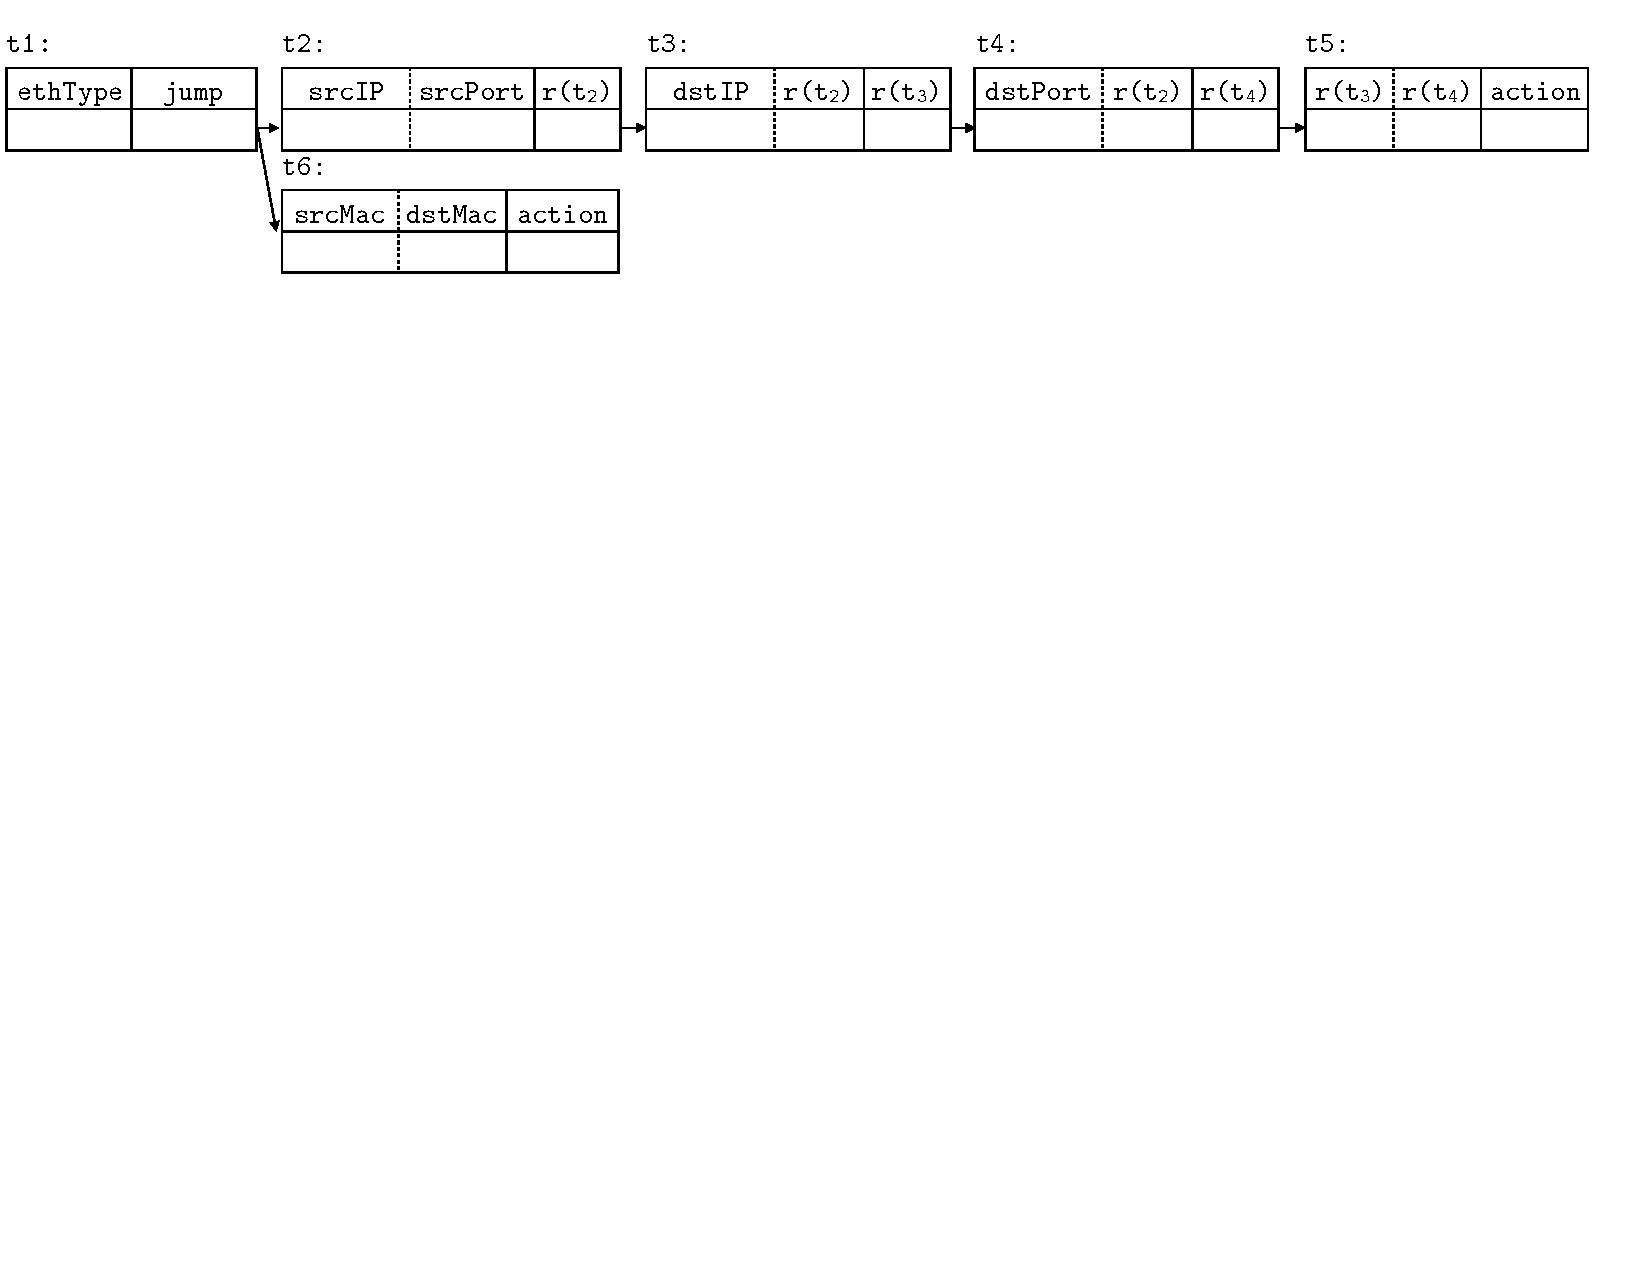
\includegraphics[scale = 0.6]{figures/figure3.pdf}
    \vspace{-2mm}
    \caption{示例数据通路, \exampledp}
    \label{cap:fig:swPipeline}
    \vspace{-2mm}
\end{figure*}

\para{示例}:我们现在给一个示例流水线\exampledp(如图~\ref{cap:fig:swPipeline}所示),来说明我们的流水线模型。要注意的是在这个例子中,一个流表的匹配列在它的左边,然后写入到它右边的寄存器中,而表中字段\texttt{output}表示这个表包含了输出路由操作。

%In \exampledp, an incoming packet starts at \exampledp's root \texttt{t1} and is passed to one of \exampledp's two ingress tables \texttt{t5} and \texttt{t6}. Therefore, \exampledp\ contains two paths, $\langle \texttt{t1}, \texttt{t2}, \texttt{t3}, \texttt{t4}, \texttt{t5} \rangle$, and $\langle \texttt{t1}, \texttt{t6} \rangle$.


%The two paths $\rho$ in \texttt{swP} are the paths in its dag from \texttt{t1} to these outputs, $\langle \texttt{t1}, \texttt{t2}, \texttt{t3}, \texttt{t4}, \texttt{t5} \rangle$ and $\langle \texttt{t1}, \texttt{t6} \rangle$.

考虑流表\texttt{t2} $\in$ \exampledp。\texttt{t2}是个精准匹配表,它的输入$I(\texttt{t2})$是\texttt{srcIP}和\texttt{srcPort},它的输出寄存器是\texttt{r(t2)}。

关于\texttt{t2}的关键计算限制是它的最大规则数$maxrules(\texttt{t2}))$和他的输出寄存器的大小$bits(\texttt{r(t2)})$。









\section{主要结果以及相关证明}
\label{sec:main-results}

%\yry{search realize and change to realize; introduce the realize symbol in main text.}
基于函数模型和流水线模型,我们现在给出关于函数$f$是否可以由流水线$pl$实现的主要结果。然后我们再给出结果的相关证明。关键的一些符号在表\ref{cap:tbl:sym-table}中写出以供参考。

\begin{table}
\centering
\begin{tabular}{| l | l |}
  \hline
  \textbf{符号} & \textbf{定义}\\
  \hline
  \hline
  \multicolumn{2}{|l|}{\textbf{路由函数相关符号}} \\
  \hline
  $f$ & 路由函数\\
  $\mathcal{F}$ & 路由函数空间\\
  $m_i$ & 数据包的匹配字段\\
  $\mathcal{M}$ & $\forall\ m_i$的集合\\
  $dom(M)$ &  $M$中有效值的域\\
  $\mathcal{R}$ &  $\forall$有效路由行为的集合\\ 
  \hline
  \hline
  \multicolumn{2}{|l|}{\textbf{流水线相关符号}} \\
  \hline
  $pl$ & 流水线\\
  $\mathcal{P}$ & 流水线函数空间\\
  $t_i$ & 流水线中的表\\
  $r(t_i)$ & $t_i$的输出寄存器\\
  $bits(r(t_i))$ & $t_i$的输出寄存器bit位长度\\
  $I(t_i)$ & $t_i$的输入\\
  $maxrules(t_i)$ & $t_i$可以包含的最大$\#$规则数\\
  \hline
\end{tabular}
\vspace{2mm}
\caption{在我们``主要结果以及相关证明"一节中使用的符号标识列表。}
\label{cap:tbl:sym-table}
\end{table}

\subsection{概述}
%---\yry{we denote xxx when f can be realized by p}--
本节的目标是得到一种系统方法来验证路由函数$f$是否可以由流水线$pl$(我们称之为$f \rightrightharpoons pl$)实现。存在的一个主要挑战是路由函数和流水线的表示方式是不同的,并且这两种表示方式都具有巨大的复杂性和多样性。可以想象将每个路由函数$f$看作函数空间$\mathcal{F}$中的一个点,将每个流水线$pl$看作函数空间$\mathcal{P}$中的一个点。 

我们的主要贡献是引入了一个创新的、统一的、规范化的函数空间$\mathcal{C}$,我们称为特征函数空间。每个路由函数$f$通过将$\tau$映射到特征函数$\tau(f) \in \mathcal{C}$来表示$f$的计算负载。另一方面,每个流水线$pl$,则被映射到一组特征函数$\kappa(pl) \subset \mathcal{C}$,表示这个流水线的一组计算能力。图~\ref{cap:fig:function-spaces}给出了这种映射结构。

%The main structure of our main result is that we can then define a third, ordered space , the space of $\forall\ c$ and produce mappings from $\mathcal{F}$ and $\mathcal{P}$ to $\mathcal{C}$ and $2^\mathcal{C}$ which we denote $\tau$ and $\kappa$ respectively. These three spaces $\mathcal{F}$, $\mathcal{P}$ and $\mathcal{C}$ and the mappings between them in are shown in Fig~\ref{fig:function-spaces}.

\begin{figure}[tbh]
    \centering
    \vspace{-1mm}
    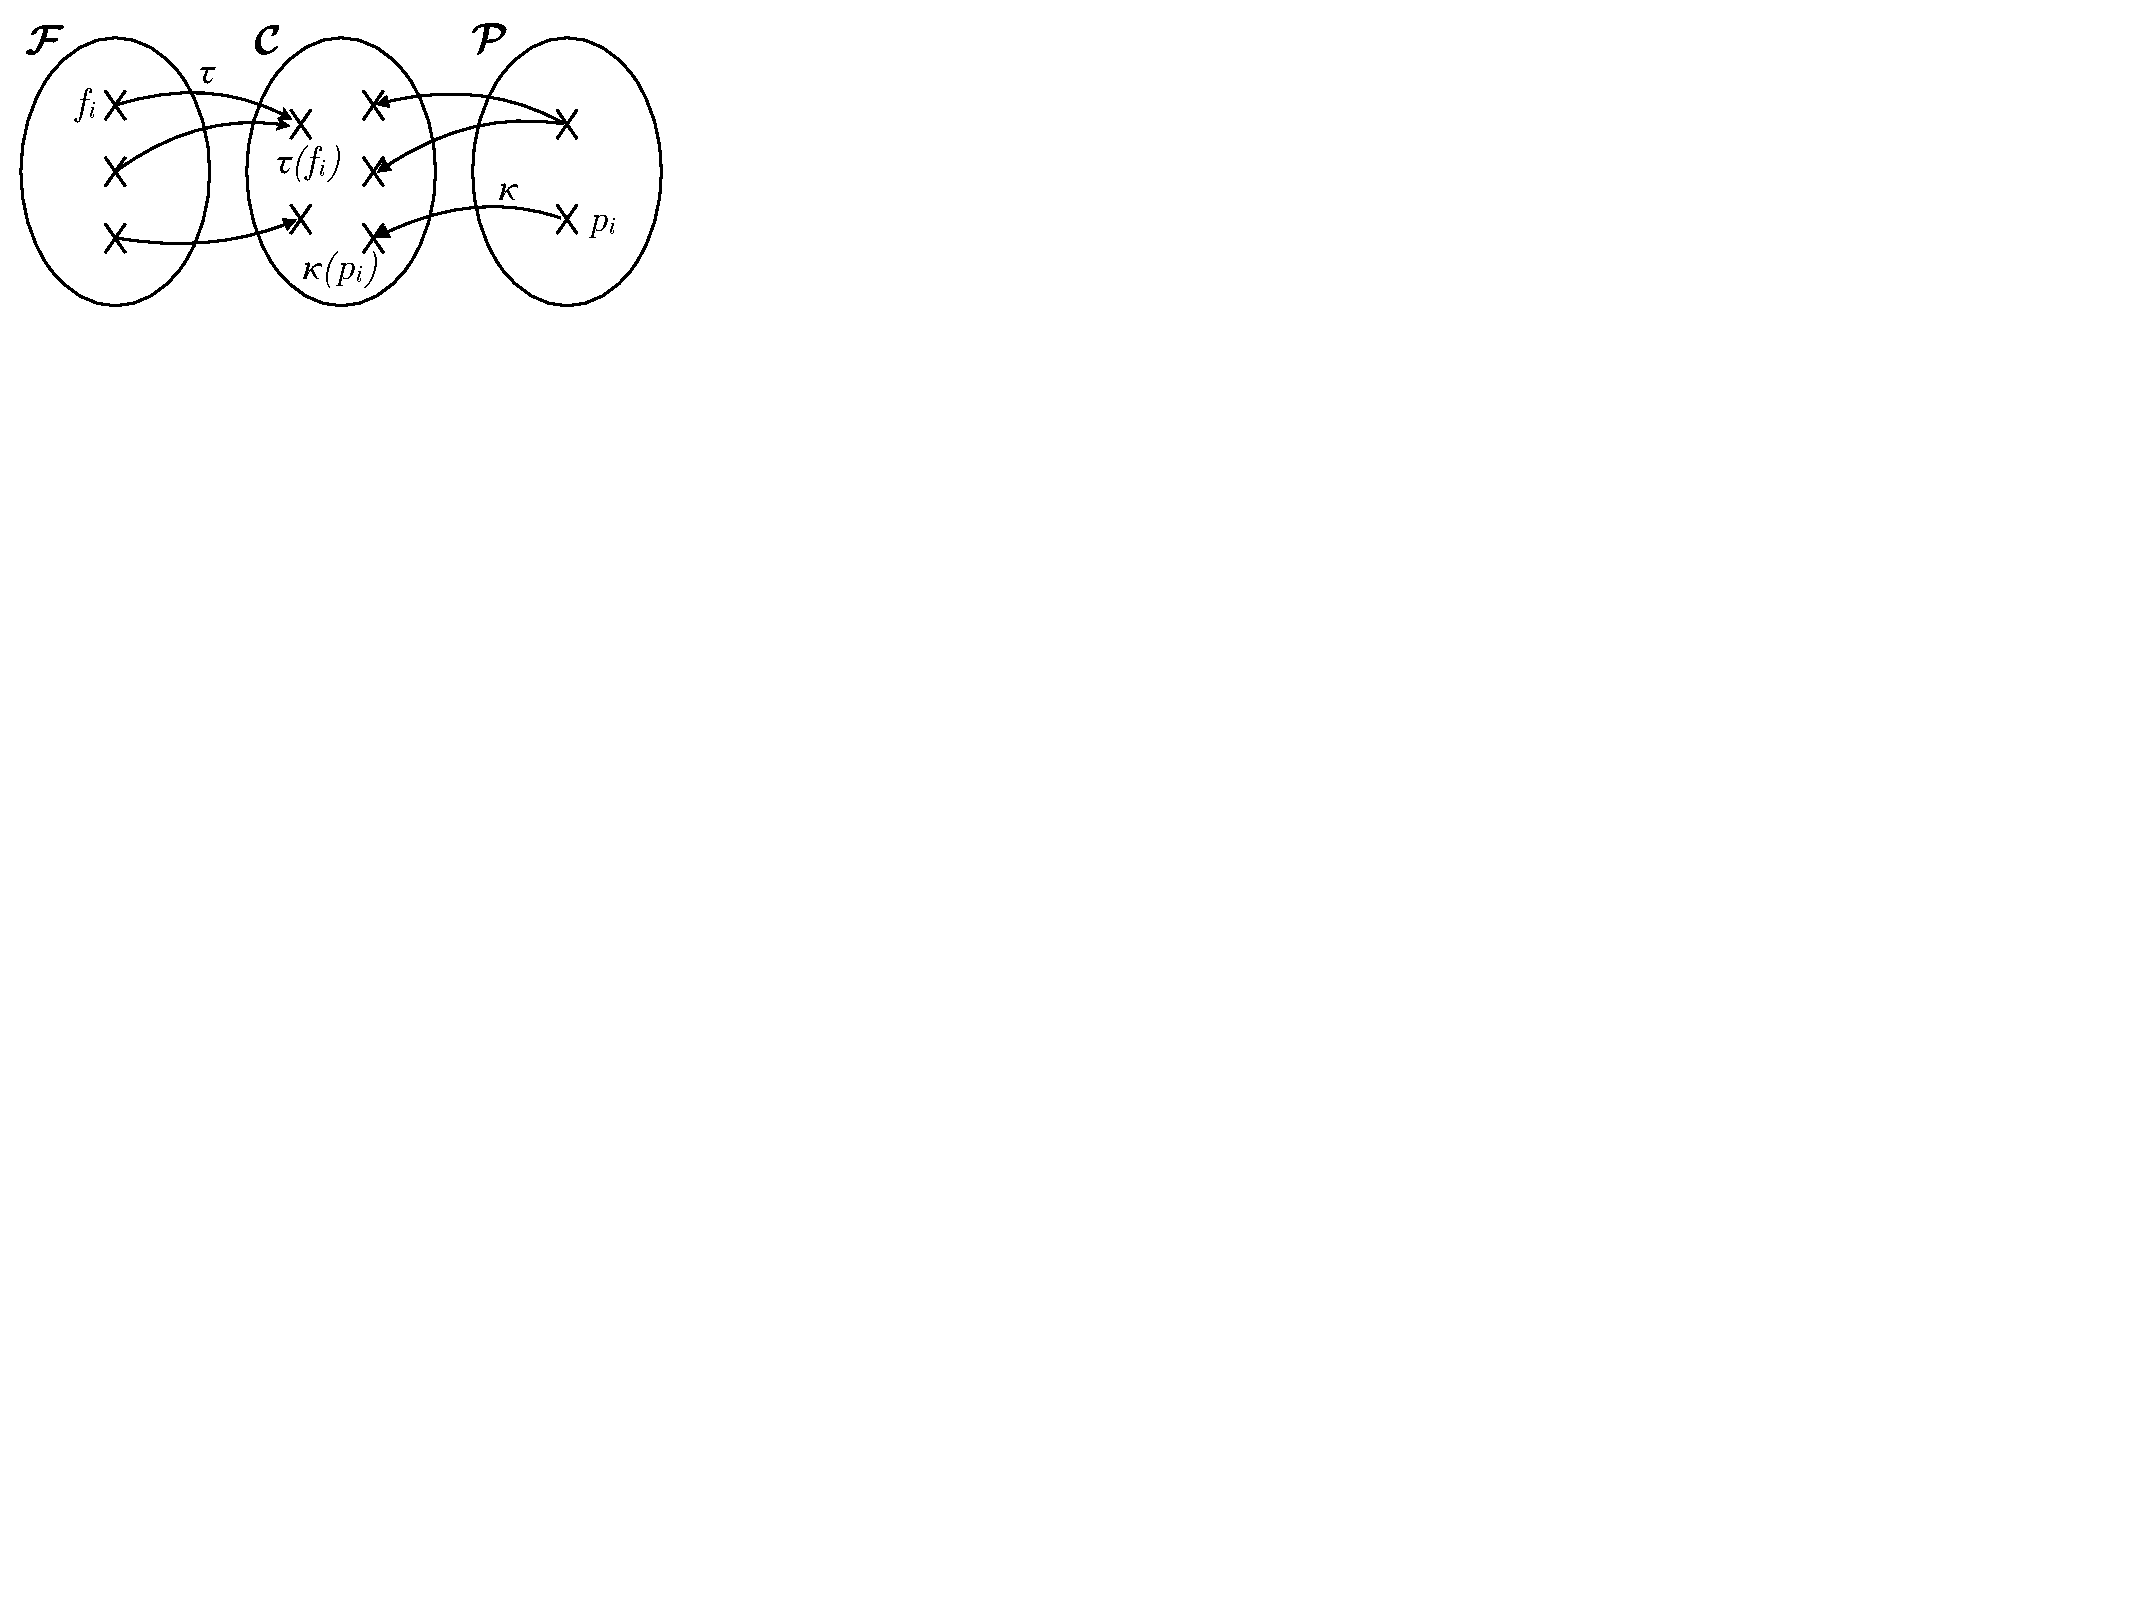
\includegraphics[clip, trim=0in 8.5in 9.8in 0in, width=2in]{figures/function-spaces.pdf}
    \vspace{-2mm}
    \caption{空间$\mathcal{F}$, $\mathcal{P}$ 和$\mathcal{C}$ 及其它们之间的映射表示。}
    \label{cap:fig:function-spaces}
    \vspace{-2mm}
\end{figure}

鉴于$\tau(f)$和$\kappa(pl)$都定义在了同一空间$\mathcal{C}$(其中$\tau(f)$对应点,$\kappa(pl)$对应一组点),人们就可以通过比较$\kappa(pl)$中的每个元素与$\tau(f)$,从而判断这个计算负载是否可以被一个计算能力``覆盖",进而导出了我们的基本容量理论,即$\exists\ c \in \kappa(pl) \geq \tau(f), f \rightrightharpoons pl$。

%Finally, we define a set of operators which act on $\mathcal{C}$ that calculate the joint characteristic functions of composed functions and networks of pipelines from their constituent functions and pipelines' characteristic functions, extending our embedding theorem to multi-pipeline networks and multi-function programs.

\subsection{特征函数}


我们首先来定义一个通用的特征函数$c$。
\begin{definition} 一个特征函数$c$是一个从数据包的匹配字段的子集$M$到一个向量的映射:  
\begin{equation*}
c(M) \overset{\Delta}{=} <scope(M),\ ec(M)>.
\end{equation*}
\end{definition}

%\yry{fix} 
我们将$c(M)$的向量的两个部分对应地称为$c(M)[scope]$和$c(M)[ec]$。

给定两个特征函数,我们可以比较它们。 

\begin{definition}我们定义$c_i$支配$c_j$, 标识为$c_i \geq c_j$ 如下:
\begin{equation*}
\begin{split}
c_i \geq c_j \overset{\Delta}{=}\ \forall\ n \in\ &\{scope, ec\},\\
&\forall\ M \in 2^\mathcal{M},\ c_i(M)[n] \geq c_j(M)[n].
\end{split}
\end{equation*}
\end{definition}

为了确保我们的容量理论,我们需要将一组特征方程和一个单独的特征方程作比较。

%Below we need ..., we define a comparator $\trianglerighteq$ between a $C \in 2^\mathcal{C}$ and a $c \in \mathcal{C}$ from Definition~\ref{def:comparator}.

\begin{definition}
一组特征方程$C_i$支配一个特征方程$c_j$, 标示为$C_i \trianglerighteq c_j$,如果存在一个$c_i \in C_i$支配$c_j$

\begin{equation*}
C_i \trianglerighteq c_j \overset{\Delta}{=} \exists\ c_i \in C_i : c_i \geq c_j.
\end{equation*}
\end{definition}
 
\subsection{路由函数的特征} 
给定特征函数的概念,我们现在导出路由$f$的特征函数,表示为$\tau(f)$。

\begin{definition}
\label{def:set-comparator}
关于数据包匹配字段$M$的一个路由函数的特征方程的范围(scope)定义为$M$中有效值域的大小:
\begin{equation*}
\tau(f)(M)[scope] \overset{\Delta}{=} dom(M)
\end{equation*}
\end{definition}

$\tau(f)(M)[ec]$是我们根据``f等价"概念建立的属性: 
%We define f-equivalence $\sim_f$ as a binary property between values of $M$ which denotes that these values cannot be distinguished by $f$. We formalize it as follows:
\begin{definition} 我们定义f等价(标识为$\sim_f$),为$M$中两个值$v_i(M)$和$v_j(M)$之间的一种联系,即不能被$f$所区分:
\begin{equation*}
\begin{split}
&v_i(M) \sim_f v_j(M) \overset{\Delta}{=} \forall\ v_k(\mathcal{M} - M) \in dom(\mathcal{M} - M),\\
&\qquad f(v_i(M), v_k(\mathcal{M} - M)) = f(v_j(M), v_k(\mathcal{M} - M)). 
\end{split}
\end{equation*}
\end{definition}



我们关于f等价的定义可以自然地导出f等价类的定义。 
\begin{definition} 一个f等价类(标识为$[v_i(M)]_f$),是一个给定的$M$中的变量$v_i(M)$的所有和它f等价的变量的组:
\begin{equation*}
[v_i(M)]_f \overset{\Delta}{=} \{v_j(M) \in dom(M) : v_i(M) \sim_f v_j(M)\}.
\end{equation*}
\end{definition}

计算等价类的数量可以得出f等价类数的概念。
 
\begin{definition}
$M$中f等价类的数量(标识为$|dom(M)/\sim_f|$),是$M$的一组等价类的基数。
\end{definition}

现在来看我们关于$\tau(f)(M)[ec]$的定义。

\begin{definition}  $M$的路由函数特征函数的ec(equivalent class)是$M$的f等价类集合的基数。 
\begin{equation*}
\tau(f)(M)[ec] \overset{\Delta}{=} |dom(M)/\sim_f|
\end{equation*}
\end{definition}
%Given these definitions, we define the characteristic function $\tau(f)$ of an $f \in \mathcal{F}$ as:

% to its characteristic function $c \in \mathcal{C}$.

\begin{definition} 路由函数的特征函数$\tau(f)$表示$f$的计算负载:
\begin{equation*}
\tau(f)(M) \overset{\Delta}{=} (dom(M),\ |dom(M)/\sim_f|).
\end{equation*}
\end{definition}




虽然$\tau(f)$非常强大,但它是不切实际的,因为直接计算等价类数需要非常大的计算。因此,我们通过定义路由函数$\tau_G(f)$的边界特征函数来限制$\tau(f)$,该函数很容易从$f$的DFG导出。该函数刻画了$f$的计算负载的一个上界: $\tau_G(f)$支配$\tau(f)$。

$\tau_G(f)[scope]$的定义如之前所述。然而,我们不计算$\tau_G(f)[ec]$,而是用$G_f$(即$f$的DFG)中特定的顶点割值来确定其上限。我们现在开始说明这个割值。


\begin{definition} 设$V_f(M)$是$G_f$中的点$m_i \in M$,$D_f(M)$是从$V_f(M)$派生的$G_f$中的点。
    \vspace{2mm}
    $M$的顶点最小割集,$G_f.vertexMinCut(M)$,是将$V_f(M)$从$D_f(\mathcal{M} -M)$中分离出来的最小割集中顶点的权重的乘积。
\end{definition}



给定这个割集,我们定义$\tau_G(f)$如下:



\begin{definition} 一个路由函数的特征函数$\tau_G(f)$刻画$f$的计算负载上限; $\tau_G(f)$支配$\tau(f)$:
\begin{equation*}
\tau_G(f)(M) \overset{\Delta}{=} (dom(M),\ G_f.vertexMinCut(M)).
\end{equation*}
\end{definition}

\para{示例}: 现在用我们的示例路由函数\texttt{onPkt}来说明这些概念。

考虑\texttt{onPkt}的匹配字段\texttt{srcIP}和\texttt{srcPort}。每个都只被读取一次:在\texttt{L4}上,由布尔函数\texttt{isVerified}读取。因此,虽然\texttt{srcIP}和\texttt{srcPort}可能分别有许多f等价类,(\texttt{srcIP}, \texttt{srcPort})只有两个:\texttt{isVerified}的值计算为$0$和它的值计算为$1$。

假设\texttt{onPkt}是一个小型商业网络的路由函数,其外层是一个连接有$50$个主机的NAT,每个主机运行着一些受限制的应用,这个限制是指只能使用$200$个标准端口。给定这个条件下,$dom(\texttt{srcIP}, \texttt{srcPort}) = 10000$,以及$\tau(\texttt{onPkt})(\texttt{srcIP}, \texttt{srcPort}) = (10000, 2)$。

虽然(\texttt{srcIP}, \texttt{srcPort})的等价类数是直接的,但\texttt{onPkt}输入的大多数其他子集的等价类数并不明显。因此,我们将$\tau(\texttt{onPkt})$ 用$\tau_G(\texttt{onPkt})$约束,它的计算使用\texttt{onPkt}的DFG($G_{\texttt{onPkt}}$)。如图~\ref{cap:fig:onpkt-dfg}所示。


%While finding the equivalence class number of (\texttt{srcIP}, \texttt{srcPort}) is straightforwards, the number of equivalence classes of other subsets of \texttt{onPkt}'s inputs such as (\texttt{srcIP}, \texttt{srcPort}, \texttt{dstIP}) is less obvious, making it difficult to calculate $c_{e,\texttt{onPkt}}$. Fortunately, we can calculate $c_{\texttt{onPkt}}$ more simply by generating \texttt{onPkt}'s DFG $G_{\texttt{onPkt}}$, shown in Fig.~\ref{fig:onpkt-dfg}.

\begin{figure}[tbh]
    \centering
    %\vspace{-1mm}
    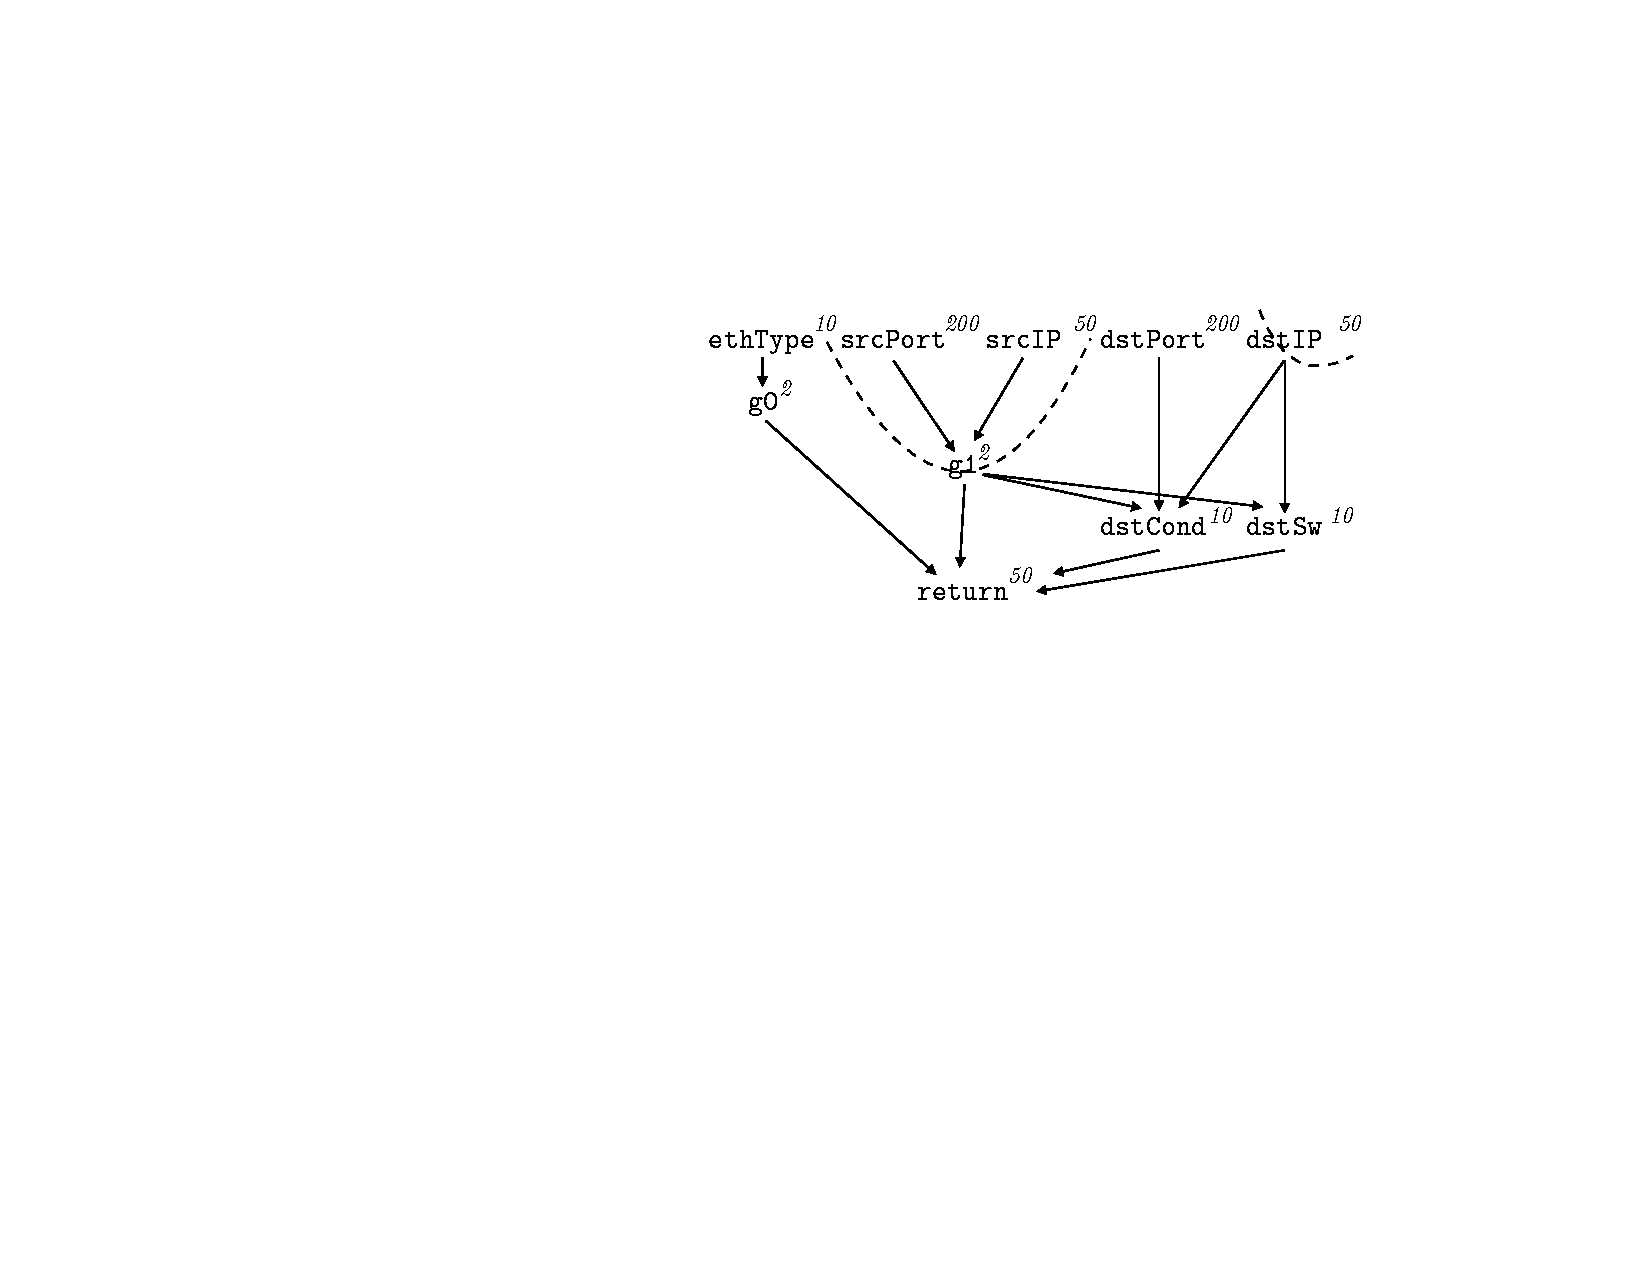
\includegraphics[scale = 0.6]{figures/figure5.pdf}
    %\vspace{-2mm}
    \caption{路由函数\texttt{onPkt}的DFG $G_{\texttt{onPkt}}$和割集$(\texttt{srcIP}, \texttt{srcPort}, \texttt{dstPort})$}
    \label{cap:fig:onpkt-dfg}
    %\vspace{-2mm}
\end{figure}

%In $G_{\texttt{onPkt}}$, vertices such as \texttt{dstSw} correspond to \texttt{onPkt}'s variables, edges such as (\texttt{dstIP}, \texttt{dstSw}) imply that the source vertex \texttt{dstIP} is used in the target vertex \texttt{dstSw}'s assignment, and vertex weights such as $w(\texttt{srcIP}) = 50$ indicate their vertices' domain.

我们考虑\texttt{onPkt}的输入为(\texttt{srcIP}, \texttt{srcPort}, \texttt{dstIP})的等价类数量。我们取它们的点和\texttt{onPkt}的其他输入: (\texttt{ethType}, \texttt{dstPort},\texttt{g0}, \texttt{dstCond}, \texttt{return})派生的每个点之间的$G_\texttt{onPkt}$中的顶点最小割集。图~\ref{cap:fig:onpkt-dfg}中用虚线表示了这个顶点最小割集。


%In $G_{\texttt{onPkt}}$, $G_{\texttt{onPkt}}.vertexMinCut(($\texttt{srcIP}, \texttt{srcPort}, \texttt{dstIP}$))$ is the product of vertex min cut weights between (\texttt{srcIP}, \texttt{srcPort}, \texttt{dstIP}) and the set of vertices descended from the remainder of \texttt{onPkt}'s inputs (\texttt{ethType}, \texttt{dstPort}): (\texttt{ethType}, \texttt{dstPort}, \texttt{g0}, \texttt{dstCond}, \texttt{return}), indicated by the dotted line in Fig.~\ref{fig:onpkt-dfg}. 

该割集中的顶点(\texttt{g1}, \texttt{dstIP})的权重为$50$和$2$,因此$\tau_G(\texttt{srcIP}, \texttt{srcPort}, \texttt{dstIP}) = (50000,\ 100)$。



\subsection{流水线的特性}
我们现在定义流水线$pl$的特征函数集$\kappa(pl)$。我们从定义通过流水线$pl$的路径$\rho$开始。

%\noindent{\em Overview}:??

\begin{definition}
一个路径 $\rho$,在$pl$中是一个通过$pl$的有向无环图的路径$\langle t_1, ..., t_n \rangle$ ,其中$t_1$是$pl$的根表,$t_n$是$pl$的出口表。

\end{definition}

作为示例,\exampledp 有两个路径$\langle \texttt{t1}, \texttt{t2}, \texttt{t3}, \texttt{t4}, \texttt{t5} \rangle$和$\langle \texttt{t1}, \texttt{t6} \rangle$,我们用$\rho_{L2}$和$\rho_{L3}$分别表示。

我们定义,$\forall\ \rho \in pl,\ \kappa_\rho(pl)$是一个流水线中一条路径的特征方程。


\begin{definition} $pl$的特征方程组$\kappa(pl)$是$\forall\ \rho \in pl$的集合:
\begin{equation*}
\kappa(pl)(M) \overset{\Delta}{=} \{c \in \mathcal{C} : c = \kappa_\rho(\rho)\ \forall\ \rho \in pl\}.
\end{equation*}
\end{definition}

我们现在通过引入以下定义来构造路径$\rho$的特征函数:

\begin{definition} 表$t_i \in \rho$的{\em 输入闭包$\bar{M}_\rho(t_i)$}是$t_i$可以获得信息的输入集合:
\begin{equation*}
\begin{split}
\bar{M}_\rho(t_i) \overset{\Delta}{=} \{m_i \in \mathcal{M} :\ &m_i \in I(t_i)\ \vee\\ &m_i \in \bar{M}_\rho(t_j)\ s.t.\ r(t_j) \in I(t_i)\}.
\end{split}
\end{equation*}
\end{definition}

%Next, we define the closure set, $\bar{\bar{M}}_\rho(M)$ of a $\rho$ as:
\begin{definition} $\rho$的$M$的{\em 闭包$\bar{\bar{M}}_\rho(M)$}是 由$t_i \in \rho$与输入闭包$M$组成的。
\begin{equation*}
\bar{\bar{M}}_\rho(M) \overset{\Delta}{=} \{t_i \in \rho : \bar{M}_\rho(t_i) = M\}. 
\end{equation*}
\end{definition}

通过这些定义,我们现在定义$\rho$的特征方程如下:
\begin{definition} {\em $\rho$的特征函数$\kappa_\rho(\rho)$}表征了$\rho$的计算容量。

$\kappa_\rho(\rho)[scope]$是$\rho$可以读取的$M$的最大数量,$\kappa_\rho(\rho)[ec]$是$\rho$可以分辨的$M$的等价类的最大数量。

\begin{equation*}
\begin{split}
&\kappa_\rho(\rho)(M) \overset{\Delta}{=}\\
&\begin{cases}
\bar{\bar{M}}_\rho(M) \neq \emptyset \quad \quad (min[maxrules(t_i) : t_i \in \bar{\bar{M}}_\rho(M)],\\
\quad \quad \quad \quad \quad \quad \quad \quad  min[2^{bits(r(t_i))} : t_i \in \bar{\bar{M}}_\rho(M)])\\
\bar{\bar{M}}_\rho(M) = \emptyset \wedge \exists\ m_i \in M :\\
m_i \notin \bigcup_{t_i \in \rho} \bar{M}(t_i, \rho)\  \quad \quad \quad \quad \quad (1, 1)\\
otherwise, \quad \quad \quad \quad \quad \quad \quad \ \ \ \ \, \, \,  (\mathrm{T}, \mathrm{T}). %(\intercal, \intercal)
\end{cases}
\end{split}
\end{equation*}
\end{definition}

\para{示例}: 与之前一样,我们使用示例流水线\exampledp 直观地说明流水线的特征函数。

\exampledp{}包含两个$\rho$: $\rho_{\texttt{L2}}$和$\rho_{\texttt{L3}}$。考虑表\texttt{t4},仅包含在$\rho_{\texttt{L3}}$中。由于\texttt{t4}读取\texttt{dstIP}和\texttt{r(t2)},而\texttt{t2}依次读取\texttt{srcIP}和\texttt{srcPort},因此输入闭包$\bar{M}_{\rho_{\texttt{L3}}}(\texttt{t4})$为(\texttt{srcIP}, \texttt{srcPort}, \texttt{dstIP})。闭包 $\bar{\bar{M}}_{\rho_\texttt{L3}}(\texttt{srcIP}, \texttt{srcPort}, \texttt{dstIP})$ 关于\texttt{t4}在$\rho_{\texttt{L3}}$的输入是$\{\texttt{t4}\}$。


因此,$\kappa_{\rho_{\texttt{L3}}}(\bar{M}_{\rho_{\texttt{L3}}})$ $=$ $\kappa_{\rho_{\texttt{L3}}}(\texttt{srcIP}, \texttt{srcPort}, \texttt{dstIP})$ $=$ $(maxRules(\texttt{t4}),$ $2^{bits(r(\texttt{t4}))})$. 在\texttt{t4}有$2^{20}$规则数并且一个$16$bit输出寄存器这种情况下, $\kappa_{\rho_{\texttt{L3}}}(\bar{M}_{\rho_{\texttt{L3}}}) = (2^{20}, 2^{16})$.

进一步,我们考虑\exampledp{}的匹配域的子集$(\texttt{srcMac},\ \texttt{dstMac})$。$\rho_{\texttt{L3}}$并不包含\texttt{srcMac}以及\texttt{dstMac},因此它只可以实现不包含\texttt{srcMac}以及\texttt{dstMac}的函数(或赋值为常数)。常数只有一个值,一个等价类。因此,对于任何输出包含\texttt{srcMac},$\kappa_{\rho_{\texttt{L3}}}$的值为$(1, 1)$。


%Further, consider the subset of \exampledp's match fields $(\texttt{srcMac},\ \texttt{dstMac})$. $\rho_{\texttt{L3}}$ does not contain the inputs \texttt{srcMac} or \texttt{dstMac} and thus it can only realize functions that contain them in the unlikely event that all are constants.  Constants have domain $1$ and $1$ equivalence class. Thus the value of $\kappa_{\rho_{\texttt{L3}}}$ for any set of outputs containing \texttt{srcMac} is $(1, 1)$.

最后,我们考虑\exampledp{}的匹配域的子集$(\texttt{srcIP},\ \texttt{srcPort})$。\texttt{srcIP}和\texttt{srcPort}都被$\rho_{\texttt{L3}}$所读,但$(\texttt{srcIP},\ \texttt{srcPort})$并不是任何$t_i \in \rho_{\texttt{L3}}$的输入闭包。在这种情况下,在判断数据通路的实现问题上不需要考虑$(\texttt{srcIP},\ \texttt{srcPort})$,因此,$\kappa_{\rho_{\texttt{L3}}}(\texttt{srcIP},\ \texttt{srcPort}) = (\mathrm{T}, \mathrm{T})$,表示我们在和路由函数的$\tau$比较时可以跳过。

%Finally, consider the subset of \exampledp's match fields $(\texttt{srcIP},\ \texttt{srcPort})$. \texttt{srcIP} and \texttt{srcPort} are both read by $\rho_{\texttt{L3}}$, but $(\texttt{srcIP},\ \texttt{srcPort})$ is not an input closure of any $t_i \in \rho_{\texttt{L3}}$. In this case, it is not necessary to consider $(\texttt{srcIP},\ \texttt{srcPort})$ to verify realizability, and thus $\kappa_{\rho_{\texttt{L3}}}(\texttt{srcIP},\ \texttt{srcPort}) = (\intercal, \intercal)$, indicating that we can skip this field during comparison with a routing funciton's $\tau$.


\subsection{数据通路编程容量理论}
结合前面关于路由函数和流水线以及它们特征函数的定义,我们最终得到了我们的核心结论:给定的$f$是否可以在给定的$pl$中实现的一个充分条件。

\begin{theorem}[流水线实现定理] 当$\kappa(pl)$(即$pl$的特征函数集)支配$\tau(f)$(即$f$的特征函数)时,一个路由函数$f$可以在流水线$pl$上实现。我们有:
\begin{equation*}
\kappa(pl) \trianglerighteq \tau(f) \Rightarrow f \rightrightharpoons pl.
\end{equation*}
\end{theorem}

作为推论,因为$\tau_G(f) > \tau(f)$,流水线实现定理可以推广到$\tau_G(f)$。

\para{示例}: 我们使用\texttt{onPkt}和\exampledp 来说明我们的流水线实现定理。具体来说,我们的流水线实现定理指出$\kappa(\exampledp) \trianglerighteq \tau(\texttt{onPkt}) \Rightarrow \exampledp \rightrightharpoons \texttt{onPkt}$。

进一步,当$\kappa_\rho(\rho_{\texttt{L2}}) > \tau_G(\texttt{onPkt})$或者$\kappa_\rho(\rho_{\texttt{L3}}) > \tau_G(\texttt{onPkt})$时,$\kappa(\exampledp) \trianglerighteq \tau(\texttt{onPkt})$为真。我们通过比较每对特征函数给出的每个向量的每个分量来验证每个条件。举例来说,$\tau(\texttt{onPkt})(\texttt{srcIP},$ $\texttt{srcPort},$ $\texttt{dstIP}$) $ = (50000,\ 100)$,  $\kappa_\rho(\rho_{\texttt{L3}})(\texttt{srcIP},$ $\texttt{srcPort},$ $\texttt{dstIP}$) $ = (2^{20}, 2^{16})$,因此输入集(\texttt{srcIP}, \texttt{srcPort}, \texttt{dstIP})不会阻碍\texttt{onPkt}在$\rho_{\texttt{L3}}$上实现。




\para{严密性}:虽然定理只提供了一个充分条件,但在一些情况下可以建立更严密的结果,即充分必要的条件。具体来说,我们有以下结果:

\begin{definition} 当$pl$的DAG没有分支时,我们称$pl$为无分支流水线。
\end{definition}

\begin{theorem}[无分支流水线实现定理] 如果$pl$是无分支流水线,且$pl$的表容量足够大,并且每个匹配字段$m_i \in \mathcal{M}$正好出现在$pl$的每一张表中,$\kappa(pl) \trianglerighteq \tau_G(f) \Leftrightarrow f \rightrightharpoons pl$.
\end{theorem}


%在章节~\ref{sec:eval1},我们通过实验评估了我们的实现定理在更一般的流水线上的严密性。



\subsection{证明}

\subsubsection{流水线实现定理的证明}

我们现在提出流水线实现定理的证明。这些证明的结构如下。首先,我们建立一种编码机制对$m \in \mathcal{M}$进行编码,并给予的足够信息,以完全执行给定的$f$。其次,在$\kappa(pl) \trianglerighteq \tau_G(f)$前提下,证明使用我们的编码的流水线可以在$pl$中实现$f$。最后,我们通过一个扩展:如果$\kappa(pl) \trianglerighteq \tau(f), f \rightrightharpoons pl$来证明$\tau_G(f) > \tau(f)$。

我们将基于$f$的$G_f$的$G_f.vertexMinCut(M)$中的点。

\begin{definition}
最小割集$\mu_f(M)$是$f$的$G_f$用$G_f.vertexMinCut(M)$分割得到的点。
\end{definition}

给定$\mu_f(M)$的值为$v_i(\mu_f(M))$且$\mu_f(M)$的值的域为$dom(\mu_f(M))$。 %We now prove the fundamental property of this set that allows us to use it as a representation:

\begin{lemma}
\label{lemma:M-to-mu}
给定$G_f.vertexMinCut(M)$,我们可以在不知道给定的值$v_i(\mu_f(M))$的情况下计算$f$。
\end{lemma}

%\begin{proof}
%We can calculate any DFG $G$'s output given the values of all of its roots because every vertex in $G$ must be descended from a subset of these roots.

%Consider the subgraph of $G_f$, $G_{f,M}$, generated by removing every vertex in $G_f$ that $\mu_f(M)$ separates from $D_f(M)$. By our definition of $G_f$, $G_f$'s output node is descended from $\forall\ m_i \in \mathcal{M}$, and thus it is always in $G_{f,M}$.

%Each of $G_{f,M}$'s roots is either a $m_j \in \mathcal{M} - M$ or some vertex in $\mu_f(M)$. Therefore, given $v_i(\mathcal{M} - M)$ and $v_j(\mu_f(M))$, we can calculate $G_{f,M}$'s output, and therefore $G_f$'s output. By the definition of a DFG, $G_f$'s output is $f$'s output, and therefore we have shown that we can calculate $f$ given $v_j(\mu_f(M))$ in lieu of $v_j(M)$.
%\end{proof}

%Further, we show that this representation is a bound on the number of equivalence classes of $M$.

%\begin{proof}
%By Lemma~\ref{lemma:domM-domMu}, $|dom(M)/\sim_f| \leq |dom(\mu_f(M))/\sim_f|$. Further, $|dom(\mu_f(M))\sim_f| < |dom(\mu_f(M))|$. Finally, $|dom(\mu_f(M))| < \prod_{\mu_f_i \in \mu_f(M)} dom(\mu_f_i)$, which is the value of $G_f.vertexMinCut(M)$.
%\end{proof}

虽然$\mu_f(M)$可以有效表示$M$的值,$v_i(M)$,但我们可以通过引入码字(codeword)的概念来对它进行压缩,从而使通过流水线的传输最大化。

\begin{definition} $f$的输入$M$的码字$\chi_f(M)$是一组整数,对应于$M$的f等价类。
\end{definition}

得到一个码字 $\in \chi_f(M)$等同于得到$M$ $v_i(M)$的值,因为可以确定地将码字映射回$v_i(M)$的等价类中的值。我们现在定义什么是``计算$M$的码字",我们将在证明中使用它:

\begin{definition} 如果我们可以计算$M$的码字$\chi_f(M)$, $\forall\ v_i(M) \in dom(M)$我们可以计算与$v_i(M)$的等价类相关联的码字。
\end{definition}

在引理~\ref{lemma:codewords}中,我们的码字给了我们一个$M$的传输要求的边界。

\begin{lemma} 
\label{lemma:codewords}
一张流表$t_i$只需要关于$M$的$log_2(\lceil |dom(\mu_f(M))|-1 \rceil)$比特的信息就可以正确执行$f$。
\end{lemma}

\begin{proof}
我们可以将任意$v_i(M) \in dom(M)$编码为$\chi_f(M)$中的码字,并且仍然可以传递足够的信息来计算$f$。如果$\mu_f(M)$可以取$|dom(\mu_f(M))|$不同的值,我们可以从集合:$0$, $...$, $|dom(\mu_f(M))|-1$中为每个值分配一个唯一的码字,最多使用$log_2(\lceil |dom(\mu_f(M))|-1 \rceil)$位来表示。
\end{proof}

\para{实现定理的证明}:基于我们对函数传输需求的描述,我们现在可以开始证明我们的实现定理。首先,我们将给出我们的关键潜在引理,引理~\ref{lemma:core-lemma},随后可以得到我们的实现定理。

\begin{lemma} 
\label{lemma:core-lemma}
如果$\forall\ t_i \in \rho = \langle t_1, ..., t_n \rangle$有$maxRules(t_i) > \tau_G(f)(\bar{M}_\rho(t_i))[dom]$,且$2^{r(t_i)} > \tau_G(f)(\bar{M}_\rho(t_i))[ec]$,那么$\forall t_i \in \rho = \langle t_1, ..., t_n \rangle$可以输出$\chi_f(\bar{M}_\rho(t_i))$到$r(t_i)$。
\end{lemma}
%
%\begin{proof}
%\noindent We prove Lemma~\ref{lemma:core-lemma} by induction. Due to space constraints, we omit the base case.
%\vspace{1mm}
%
%\noindent \textit{Inductive step:} Assume Lemma~\ref{lemma:core-lemma} is true for $\langle t_1, ..., t_k \rangle$. We show Lemma~\ref{lemma:core-lemma} is true for $\langle t_1, ..., t_{k+1} \rangle$.
%\vspace{1mm}
%
%We prove the inductive case in two stages. First, we show that if $maxRules(t_1) > \tau_G(f)(\bar{M}_\rho(t_1))[dom]$, $t_{1}$ can compute $\chi_f(\bar{M}_\rho(t_{1}))$. Second, we show that given that $t_{1}$ can compute $\chi_f(\bar{M}_\rho(t_{1}))$, if $2^{r(t_{1})} > \tau_G(f)(\bar{M}_\rho(t_{1}))[ec]$, $\chi_f(\bar{M}_\rho(t_{1}))$ can be output by $t_1$ to $r(t_{1})$.
%%We prove the inductive step with the same two stages we used to prove the base case.
%\vspace{1mm}
%
%We start by proving stage 1. $m_i \in \bar{M}_\rho(t_{k+1}) \Leftrightarrow m_i \in I(t_{k+1}) \vee m_i \in \bar{M}_\rho(t_{i}) : r(t_i) \in I(t_{k+1})$. $r(t_i) \in I(t_{k+1}) \Leftrightarrow r(t_i) \in (r(t_1), ..., r(t_{k+1}))$.
%
%By the inductive hypothesis, $r(t_i) \in (r(t_1), ..., r(t_{k+1})) \Rightarrow r(t_i)$ will contain $\chi_f(\bar{M}_\rho(t_{i}))$. Therefore, $t_{k+1}$ can read $\forall\ m_i \in \bar{M}_\rho(t_{k+1})$ from $m_i \in I(t_{k+1}) \vee r(t_i) \in I(t_{k+1})$.
%\vspace{1mm}
%
%Now, as in the base case, if a table $t_m$ is given $\forall\ m_i \in \bar{M}_\rho(t_{k+1})$, it can compute $\chi_f(\bar{M}_\rho(t_{k+1}))$ by matching on all $v_i(\bar{M}_\rho(t_{k+1})) \in dom(\bar{M}_\rho(t_{k+1}))$ if $maxRules(t_{m}) > dom(\bar{M}_\rho(t_{k+1}))$.
%\vspace{1mm}
%
%We now show how to transform $t_m$ into $t_{k+1}$ without increasing $t_m$'s rule number. $\forall\ m_i \in \bar{M}_\rho(t_{k+1})$:
%
%\begin{itemize}
% \item If $m_i \in I(t_{k+1})$, we can leave $m_i$'s column in $t_m$ alone.
%
% \item If $m_i \notin I(t_{k+1}) \Rightarrow r(t_i) \in I(t_{k+1}) : r(t_i)$ contains $\chi_f(M_j) : m_i \in M_j$. Further, $M_j \subseteq \bar{M}_\rho(t_{k+1})$. Thus, each rule in $t_m$ generates precisely one codeword in $\chi_f(M_j)$. We therefore replace $t_m$'s match field header $m_i$ with $\chi_f(M_j)$, and that each of that header's values in $t_m$'s rules with that rule's codeword in $\chi_f(M_j)$.
%\end{itemize}
%
%This transformation does not increase rule number and results in a table that only matches on headers in $I(t_k)$. Thus we have proved stage 1.
%
%%Thus we have shown $t_{k+1}$ can compute $\chi_f(\bar{M}_\rho(t_{k+1}))$ if $maxRules(t_{k+1}) > dom(\bar{M}_\rho(t_{k+1}))$, and $\tau_G(f)(\bar{M}_\rho(t_{k+1}))[dom] \leq dom(\bar{M}_\rho(t_{k+1}))$. 
%
%We now proceed to proving stage 2. $\chi_f(M)$ only requires $\lceil log_2(|M/\sim_f|) \rceil$ bits to represent it. Therefore $2^{r(t_{k+1})} > |\bar{M}_\rho(t_{k+1})/\sim_f| \Rightarrow \chi_f(\bar{M}_\rho(t_{k+1}))$ can be placed in $r(t_{k+1})$. $\tau_G(f)(\bar{M}_\rho(t_{k+1}))[ec] \leq 2^{r(t_{k+1})}$.
%\end{proof}

给出引理~\ref{lemma:core-lemma}后,我们现在可以证明实现定理了。

\begin{proof}
给定$f$和$p$,我们会证明如果 $\kappa(pl)\trianglerighteq tau(f)$, $f \rightrightharpoons pl$。考虑 $\kappa_\rho(\rho) \in \kappa(pl)$。

$\forall\ M \in \mathcal{M} : m_i \in M \rightarrow m_i \notin \bigcup_{t_i \in \rho} \bar{M}_\rho(t_i),\ \kappa_\rho(\rho)(M) = (1,\ 1)$。 因此,如果$\kappa_\rho(\rho) > \tau_G(f) \Rightarrow$ 没有被$\rho$读取的所有$m_i$会被视作常量或者根本不会被$f$读取,因此$f$是从 $\bigcup_{t_i \in \rho} \bar{M}_\rho(t_i) \rightarrow \mathcal{R}$得到的映射。 

进一步,给定$\kappa_\rho(\rho) > \tau_G(f)$ $\forall\ t_i \in \rho,\ maxRules(t_i) > \tau_G(f)(\bar{M}_\rho(t_i))[dom]$,且$2^{r(t_i)} > \tau_G(f)(\bar{M}_\rho(t_i))[ec]$,那么因此根据引理~\ref{lemma:core-lemma} $t_n$可以计算$\chi_f(\bar{M}_\rho(t_n))$。

最后,考虑到如果一个$t_i$可以计算$\chi_f(M_i)$,并且一个$f$是$dom(M_i) \rightarrow \mathcal{R}$的映射, $t_i$可以通过把$\chi_f(M_i)$中的码字映射到它关联的$f$的输出的方式,计算$f$的输出$\forall\ v_j(M_i) \in dom(M_i)$。

鉴于$t_n$是$\rho$的唯一输出, $\bar{M}_\rho(t_n) = \bigcup_{t_i \in \rho} \bar{M}_\rho(t_i)$。因此, $t_n$可以计算 $f$的输出进一步,鉴于$t_n$是一个出口表,它总是可以将此输出传递回交换机。

因此,如果$\kappa_\rho(\rho) > \tau_G(f), f \rightrightharpoons \rho$。 鉴于 $\kappa_\rho(\rho) \in k(p)$和$\rho \in pl$, 我们已经证明如果$\kappa(pl)\trianglerighteq \tau_G(f)$, $f \rightrightharpoons pl$。
\end{proof}

证明我们的实现定理所需的最后一步是证明$\tau_G(f) > \tau(f)$所以才有$\kappa(pl)\trianglerighteq \tau(f) \Rightarrow f \rightrightharpoons pl$。下面引理~\ref{lemma:domM-domMu}给出了这一步骤的要点。
 
\begin{lemma} $M$等价类的数量被$dom(\mu_f(M))$所限定。
%$|dom(M)/\sim_f| \leq |dom(\mu_f(M))\sim_f|$.
\label{lemma:domM-domMu}
\end{lemma}

\begin{proof}
通过反证法, 假设$\exists\ (f,\ M) : |dom(M)/\sim_f| > dom(\mu_f(M)$。$v_i(M)$ 在$M$中的某个等价类的每个$v_i(M)$必须生成一个 $v_i(\mu_f(M))$。根据鸽子洞原理~\cite{ajtai1988complexity},如果$M$的等价类多于$\mu_f(M)$,则来自不同等价类的$M$的两个值必须生成相同的$\mu_f(M)$。然而,根据引理~\ref{lemma:M-to-mu},$\mu_f(M)$包含关于$M$的足够信息来确定$f$的输出值,因此$M$的这两个值必须在同一等价类中,这是一个矛盾。
\end{proof}

%As a corrollary, we have shown that $G_f.vertexMinCut(M)$ bounds $M$'s equivalence classes.

\begin{corrollary} 任一$M$的f等价类的数量$G_f.vertexMinCut(M)$所限。
\label{lemma:eq-cl-approx}
\end{corrollary}

\begin{corrollary} 特征方程$\tau_G(f)$支配特征方程 $\tau(f)$。
\label{lemma:eq-cl-approx}
\end{corrollary}



因此,我们证明了我们的实现定理:$\kappa(pl)\trianglerighteq \tau_G(f) \Rightarrow f \rightrightharpoons pl$。

\subsubsection{无分支流水线实现定理的证明}

上一小节中已经证明了我们的实现定理,$\kappa(pl)\trianglerighteq \tau_G(f) \Rightarrow f \rightrightharpoons pl$,现在我们证明如果$pl$是无分支流水线,且$pl$的表容量足够大,并且每个匹配字段$m_i \in \mathcal{M}$正好出现在$pl$的每一个表中,$\kappa(pl) \trianglerighteq \tau_G(f) \Leftrightarrow f \rightrightharpoons pl$.
%
%As our realization theorem, $\kappa(p)\trianglerighteq \tau_G(f) \Rightarrow f \rightrightharpoons p$, has been proved, now we give a proof for that if $p$ is a branchless pipeline, $p$'s table size is large, and each match field $m_i \in \mathcal{M}$ appears in exactly one of $p$'s tables, $f \rightrightharpoons p \Rightarrow \kappa(p) \trianglerighteq \tau_G(f)$.
%

通过反证法,我们假设$f \rightrightharpoons pl$但存在$M$使得$\kappa(pl)(M)[ec] < \tau_G(f)(M)[ec]$(我们省略$M$的域大小因为$pl$的表足够大)。因为$f \rightrightharpoons pl$且$pl$是一个无分支流水线且每一个匹配字段$m_i \in \mathcal{M}$都正好出现在一个$pl$的流表中,因此我们有$\kappa(pl)(M)[ec] \ge \prod \kappa(pl)(m_i)[ec]$(其中$m_i \in M$)。因此我们有$\kappa(pl)(M)[ec] \ge \tau_G(f)(M)[ec]$,而这与$\kappa(pl)(M)[ec] < \tau_G(f)(M)[ec]$有矛盾。完成证明。

%We consider the contradiction that $f \rightrightharpoons p$ but there exists $M$ that $\kappa(p)(M)[ec] < \tau_G(f)(M)[ec]$ (Note that here we omit the domain size of $M$ as the $p$'s table size is large). As $f \rightrightharpoons p$ and $p$ is a branchless pipeline and each match field $m_i \in \mathcal{M}$ appears in exactly one of $p$'s tables, we can have $\kappa(p)(M)[ec] \ge \prod \kappa(p)(m_i)[ec]$ where $m_i \in M$. Then, we have $\kappa(p)(M)[ec] \ge \tau_G(f)(M)[ec]$ which has contradiction with $\kappa(p)(M)[ec] < \tau_G(f)(M)[ec]$. Therefore, we have the proof.



\section{实验评估}

我们现在对路由函数特征化的严密性(即计算出的值与真实值的差异性),路由函数特征化的时间复杂度,流水线特征化,以及流水线实现四个方面进行数值评估。所有的实验在3.5 GHz Intel i7 处理器上运行,内存为16 GB,系统为Mac OSX 10.13。

%We now evaluate the characterization of a routing function and a pipeline from the tightness, computation complexity, and output size.  and running OS X system.

\subsection{路由函数特征化的严密性}
\label{sec:eval1}

通过比较以下一组路由函数的$\tau$和$\tau_G$的一个$M$等价类的数量(即$ec(M)$),我们证明路由函数特征化的严密性。对于$\tau$的$ec(M)$计算将采用f等价类的定义进行计算。

%We have examined the tightness of characterization of a routing function by comparing the $ec(M)$, the number of equivalent classes for a set of matches $M$, from two mappings (\ie, $\tau$ and $\tau_G$) for several routing functions. The computation of $ec(M)$ for the mapping $\tau$ is based on the definition of f-equivalence which will get the exact value of the number of equivalent classes of a set of matches $M$ for a particular routing function. The routing functions we use are shown as follows :

{\small
\begin{verbatim}
\\  Routing function: simpleRoute
L1: def simpleRoute(Addr srcIP, Addr dstIP):
L2:   srcSw = hostTbl[srcIP]
L3:   dstSw = hostTbl[dstIP]
L4:   route = routeTbl[srcSw, dstSw]
L5:   return route
\end{verbatim}
}

我们的第一个函数\texttt{simpleRoute}将包的\texttt{srcIP}和\texttt{dstIP}映射到它们的主机包交换机\texttt{dstSw}和\texttt{srcSw},然后查找它们之间的路由。


%Function 1 (\texttt{simpleRoute}) reads two inputs and maps them to internal variables respectively based on a table, \texttt{hostTbl}. After that, \texttt{simpleRoute} gets the route from another table, \texttt{routeTbl}, where the key is two internal variables.

{\small
\begin{verbatim}
//  Routing Function: condRoute
L1: def condRoute(srcIP, dstIP):
L2:   srcSw = hostTbl[srcIP]
L3:   dstSw = hostTbl[dstIP]
L4:   routeCond = condTbl[srcIP, dstIP]
L5:   route = routeTbl[srcSw, dstSw, routeCond]
L6:   return route
\end{verbatim}
}
我们的第二个函数\texttt{condRoute}通过引入一个路由条件变量来扩展\texttt{simpleRoute},该变量影响路由查找。

%Function 2 (\texttt{f2}) is similar to \texttt{simpleRoute} except that there is a third table, \texttt{condTbl}, which returns an internal variable, \texttt{cond}, used as a part of the key of \texttt{routeTbl}.

{\small
\begin{verbatim}
//  Routing Function: secureRoute
L1: def secureRoute(Addr srcIP, Addr dstIP):
L2:   if (isFiltered(srcIP)):
L3:     return Drop()
L4:   else:
L5:     route = fwdTbl[dstIP]
L6:     return route
\end{verbatim}
}
我们的最后一个函数\texttt{secureRoute}将所有\texttt{srcIP}在一个过滤器列表中的数据包丢弃,并转发其余的数据包。


\para{结果}:结果见表~\ref{cap:table:table1}。具体来说,在表~\ref{cap:table:table1}中,第2列定义了\texttt{srcIP}、\texttt{dstIP}的域,第3-6列给出了每个表的输出范围$O(tbls)$,第7-10列给出了每个函数的$\tau(f)$和$\tau_G(f)$中选定字段的值。行b1(scR)和b2(scR)分别表示\texttt{secureRoute}的两个分支,L2$\to$L3和L2$\to$L4$\to$L5$\to$L6。当一个值不适用于给定函数时,我们记录N/A,当计算失败时,$\tau(f)$的值为null。

%gives the characterization results for the four functions, \texttt{simpleRoute}, \texttt{f2}, \texttt{f3}, and \texttt{onPkt}. The second column, $bits(input)$, defines the number of bits of both inputs, \ie, \texttt{srcIP}, \texttt{dstIP}; We use $\#O(t)$ to represent the number of possible output value for the table $t$; We only evaluate the equivalent class value in the output vector of characterization of a function for a particular input; The notation $b1(\texttt{f3})$ represents the branch 1 in \texttt{f3}, \ie, L1$\to$L2, while $b2(\texttt{f3})$ represents the branch 2 in \texttt{f3}, \ie, L1$\to$L3$\to$L4$\to$L5.

在我们对\texttt{simpleRoute}和\texttt{condRoute}的计算中,除$O(\texttt{condTbl})$ = 1的特殊情况外,$\tau$和$\tau_G$的结果在任何情况下都几乎相同。值得注意的是,我们的$\tau(f)$和$\tau_G(f)$值不受$routeTbl$ $O(\texttt{routeTbl})$范围的影响。这说明当\texttt{hostTbl}($s_1$)不等于\texttt{hostTbl}($s_2$)时($s_1$和$s_2$是$srcIP$的两个值),$s_1 \sim_f s_2$的概率非常小。


%From the evaluation of simpleRoute and f2, we can see the result of $\tau$ and $\tau_G$ are almost the same except an extreme case where $\#O(\texttt{condTbl})$ = 1. Also, the results are not influenced by $\#O(\texttt{routeTbl})$, which can be observed from the first three rows in the table. This is because, considering $s_1$ and $s_2$ as two values of $srcIP$, if \texttt{hostTbl}($s_1$) is not equal to \texttt{hostTbl}($s_2$), then the chance of $s_1 \sim_f s_2$ is very small.

进一步发现,带有控制语句的函数:\texttt{secureRoute}以及\texttt{onPkt},在$\tau$和$\tau_G$之间有一个很大的差距。这表明$\tau_G$的界在有分支程序上是较松的。然而,正如行b1(scR)和行b2(scR)所示,我们可以对程序的每一个分支计算特征函数来解决这个问题。对于每一个分支(如b1(scR)和行b2(scR)所示),$\tau$和$\tau_G$仍然保持着严密性。

%For the functions with control statements, such as f3, the results of $\tau$ and $\tau_G$ have a large gap. However, in this case, we can split the function into different branches. For each branch, the result of $\tau$ and $\tau_G$ maintains the tightness, which is shown in the rows with $b1(\texttt{f3})$ and $b2(\texttt{f3})$ in Table~\ref{table:table1}. Also, we evaluate the example routing function \texttt{onPkt}, and the result is shown in the last row in the table. Need to mention that, both $\tau$(f)(\texttt{srcIP}) and $\tau$(f)(\texttt{dstIP}) are null means that the computation time is too long to compute the result.

\begin{table*}[t]
\centering
\scalebox{0.75}{
\begin{tabular}{ | l | l | l | l | l | l | l | l | l | l | }
    \hline
    $f$ & $bits(IP)$ & $O(\texttt{hostTbl})$ & $O(\texttt{routeTbl})$ & $O(\texttt{condTbl})$ & $O(\texttt{fwdTbl})$ & $\tau$(f)(\texttt{srcIP}) & $\tau$(f)(\texttt{dstIP}) & $\tau_G$(f)(\texttt{srcIP}) & $\tau_G$(f)(\texttt{dstIP}) \\
    \hline   
    smplR & 10 & 100 & 2 & N/A & N/A  & 100 & 100 & 100 & 100 \\
    smplR & 10 & 100 & 30 & N/A & N/A & 100 & 100 & 100 & 100 \\
    smplR & 10 & 100 & 5000 & N/A & N/A & 100 & 100 & 100 & 100 \\
    smplR & 12 & 100 & 30 & N/A & N/A & 100 & 100 & 100 & 100 \\
    smplR & 10 & 200 & 30 & N/A & N/A & 200 & 200 & 200 & 200 \\
    condR & 10 & 100 & 30 & 50 & N/A & 1024 & 1024 & 1024 & 1024 \\
    condR & 10 & 100 & 30 & 5 & N/A & 1024 & 1024 & 1024 & 1024 \\
    condR & 10 & 100 & 30 & 1 & N/A & 100 & 100 & 1024 & 1024 \\
    scR & 10 & N/A & N/A & N/A & 100 & 2 & 100 & 2 & 1024 \\
    b1(scR) & 10 & N/A & N/A & N/A & N/A & 1 & N/A & 1 & N/A \\
    b2(scR) & 10 & N/A & N/A & N/A & 100 & 1 & 100 & 1 & 100 \\
    \texttt{onPkt} & 32 & 100 & 30 & 50 & N/A & null & null & $2^{32}$ & $2^{32}$ \\
    \hline
  \end{tabular}
  }
\vspace{1mm}
\caption{不同统计量下路由函数的特征化结果}
\label{cap:table:table1}
\end{table*}


\subsection{路由函数特征的时间复杂度}

我们现在比较给定路由函数计算$\tau$和$\tau_G$所需的时间。如上一实验所述,$\tau$的计算将基于f等价类的定义。我们使用\texttt{simpleRoute}进行测试。其中$O(\texttt{hostTbl})$ = 100,并改变输入范围(即输入比特位)和\texttt{routeTbl}的大小。
%
%We now examine the computing complexity of characterization of a routing function by comparing the computation time of two mappings (\ie, $\tau$ and $\tau_G$) for the same function. As the same with the first evaluation, the computation of $\tau$ is based on the definition of f-equivalence. We run our tests using \texttt{simpleRoute} where the size of \texttt{hostTbl} = 100 with different size of domain of input (\ie, the bits of input) and different size of \texttt{routeTbl}.
%

\para{结果}:图~\ref{cap:fig:eval-ct}说明了随着输入以及\texttt{routeTbl}的变大,$\tau_G$的计算具有良好的可拓展性,即运算时间不改变。其中图~\ref{cap:fig:eval-ct:a}表示的是在固定\texttt{routeTbl}大小为100的情况,而图~\ref{cap:fig:eval-ct:b}表示的是固定输入外围为6的情况。从图~\ref{cap:fig:eval-ct:a}可以看出,随着输入比特位的变大,$\tau$的计算时间呈指数级增长而$\tau_G$基本不变。从图~\ref{cap:fig:eval-ct:b}可以看出,随着\texttt{routeTbl}的变大,$\tau$的计算时间同样呈指数级增长而$\tau_G$基本不变。这是由于$\tau_G$的计算只依赖于DFG而$\tau$需要对每个不同输入执行函数。

%Fig.~\ref{fig:eval-ct} shows the scalability of $\tau_G$ as input size and \texttt{routeTbl} size grows. Specifically, Fig.~\ref{fig:eval-ct:a} gives the result with fixed \texttt{routeTbl} size which equals 100, and Fig.~\ref{fig:eval-ct:b} gives the result with fixed input size which equals 6. As shown in Fig.~\ref{fig:eval-ct:a}, as the bit length of \texttt{srcIP} and \texttt{dstIP} increases, $\tau_G$'s computation time remains constant while $\tau$'s computation time grows in exponential order. And as illustrated in Fig.~\ref{fig:eval-ct:b}, as \texttt{routeTbl} size grows, the $\tau_G$'s computation time still remains constant while $\tau$'s computation time grows in polynomial level. This is because the computation of $\tau_G$ only requires the cuts of DFG which can be done in a very fast way but the computation of $\tau$ requires the execution of function for every possible input.



\begin{figure}
  \centering
  % \subfigure[输入比特位长度变化]{
  %   \label{cap:fig:eval-ct:a} 
  %   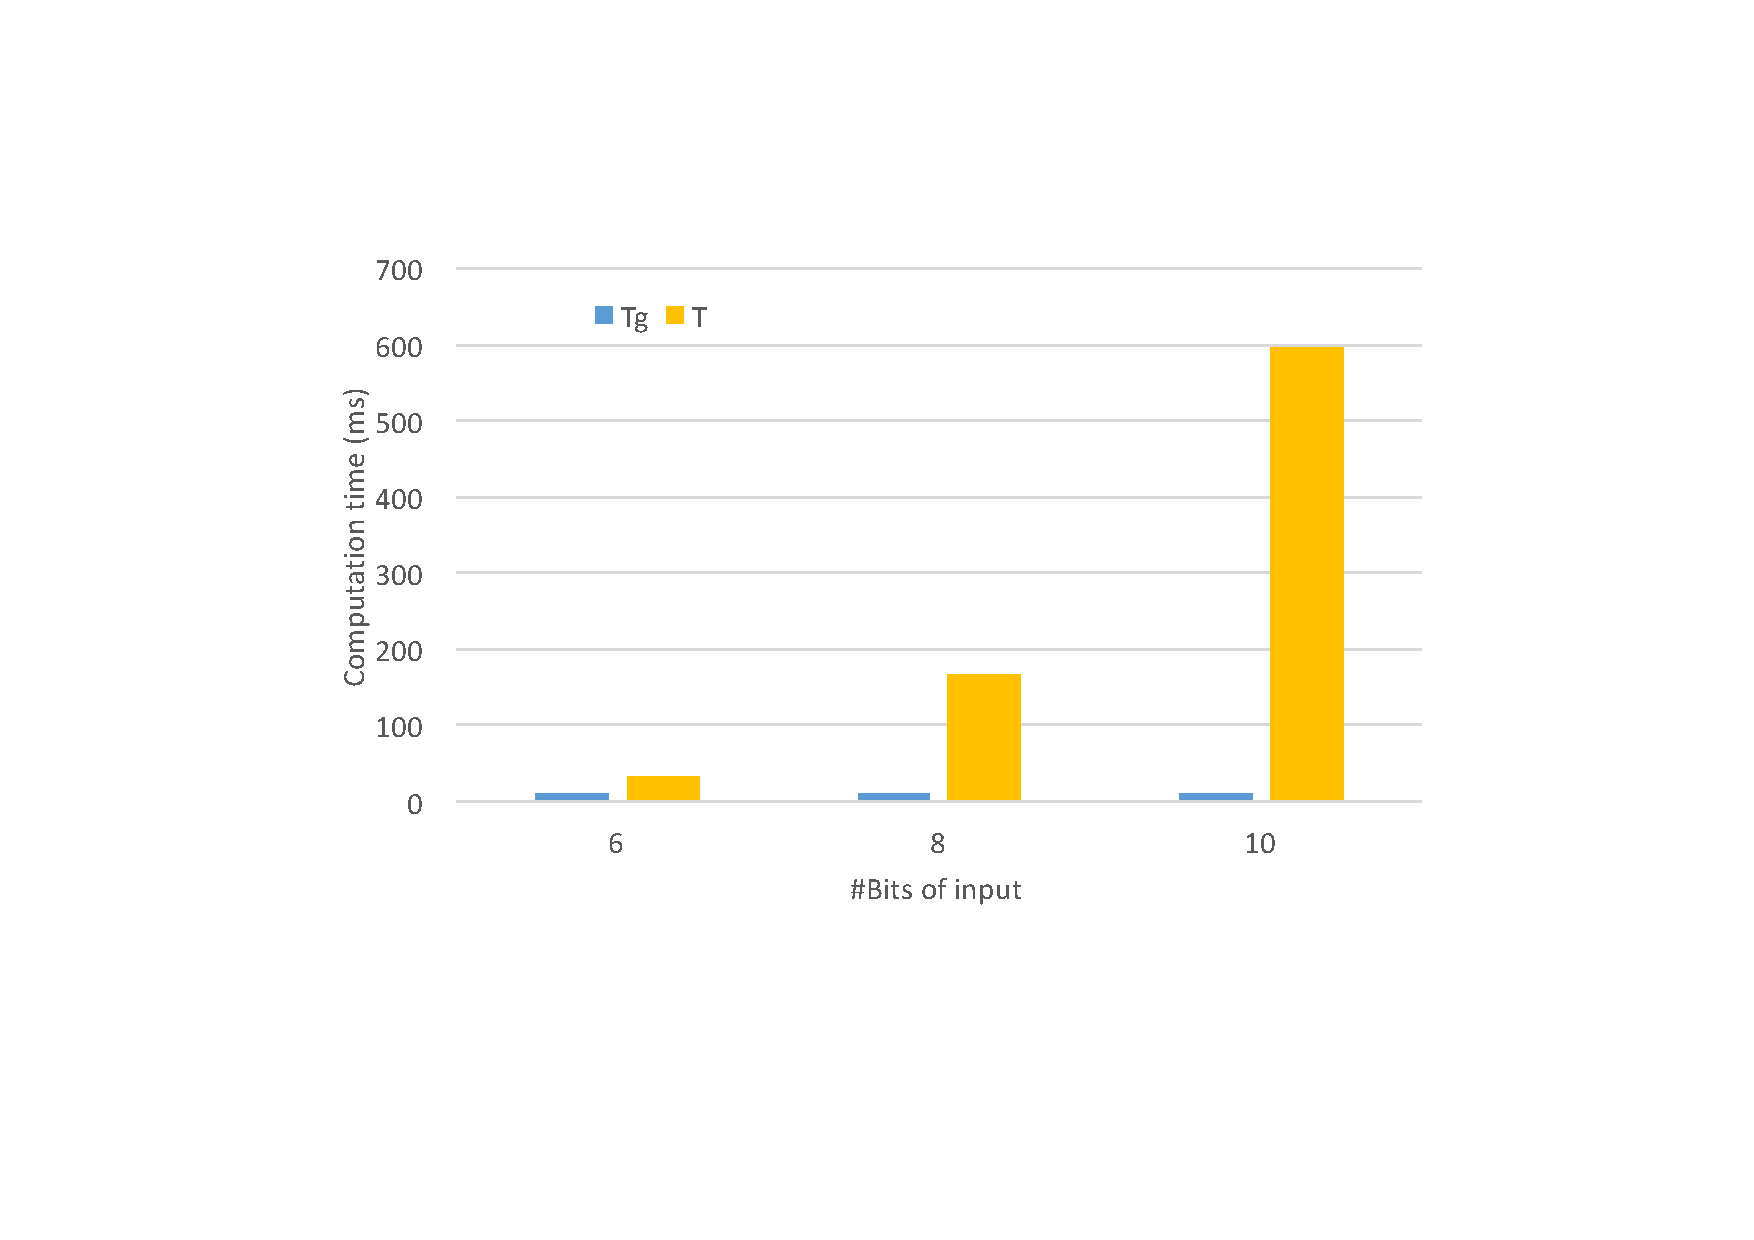
\includegraphics[width=0.4\textwidth]{figures/figure-eval-t1.pdf}}

  \begin{subfigure}[b]{0.4\textwidth}
      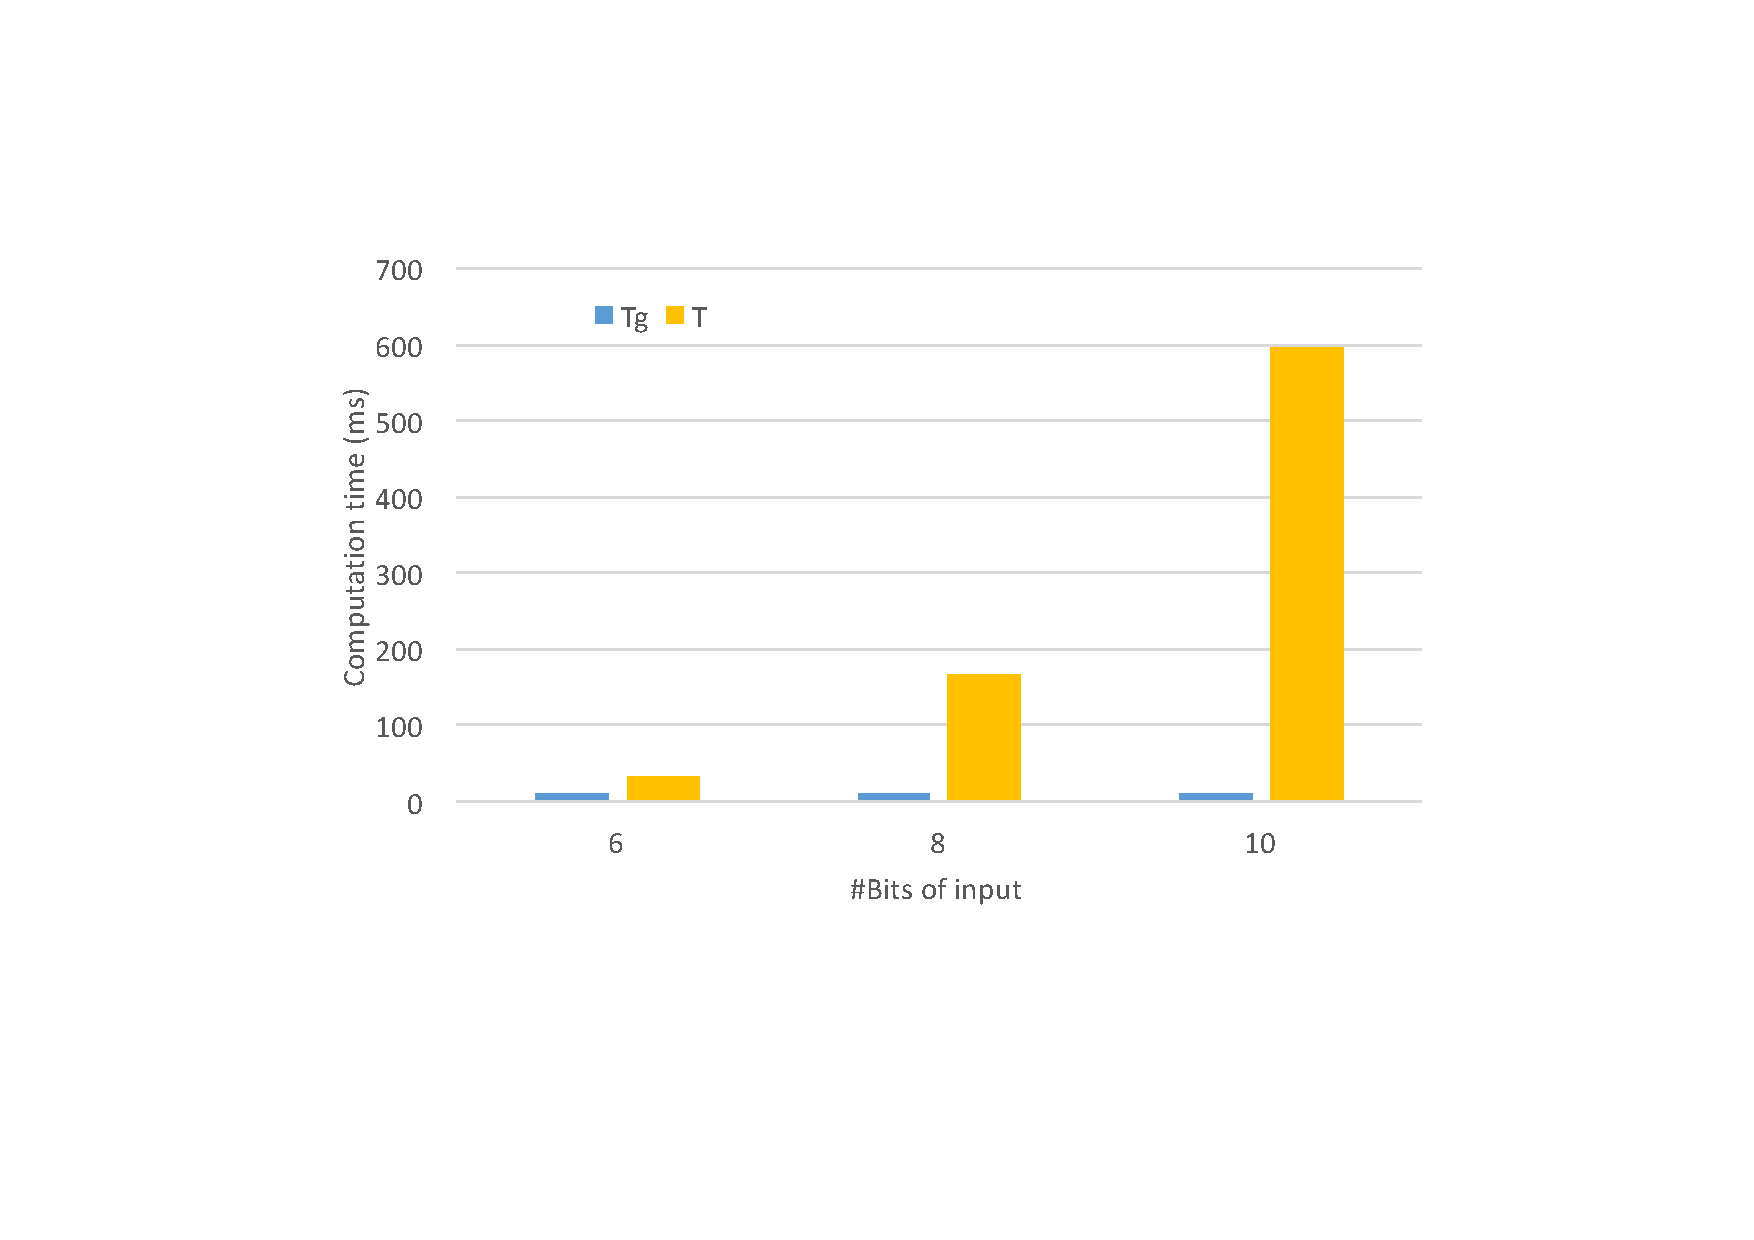
\includegraphics[width=\textwidth]{figures/figure-eval-t1.pdf}
      \caption{输入比特位长度变化}
      \label{cap:fig:eval-ct:a}
  \end{subfigure}

  \hspace{1in}
  % \subfigure[表大小变化]{
  %   \label{cap:fig:eval-ct:b}
  %   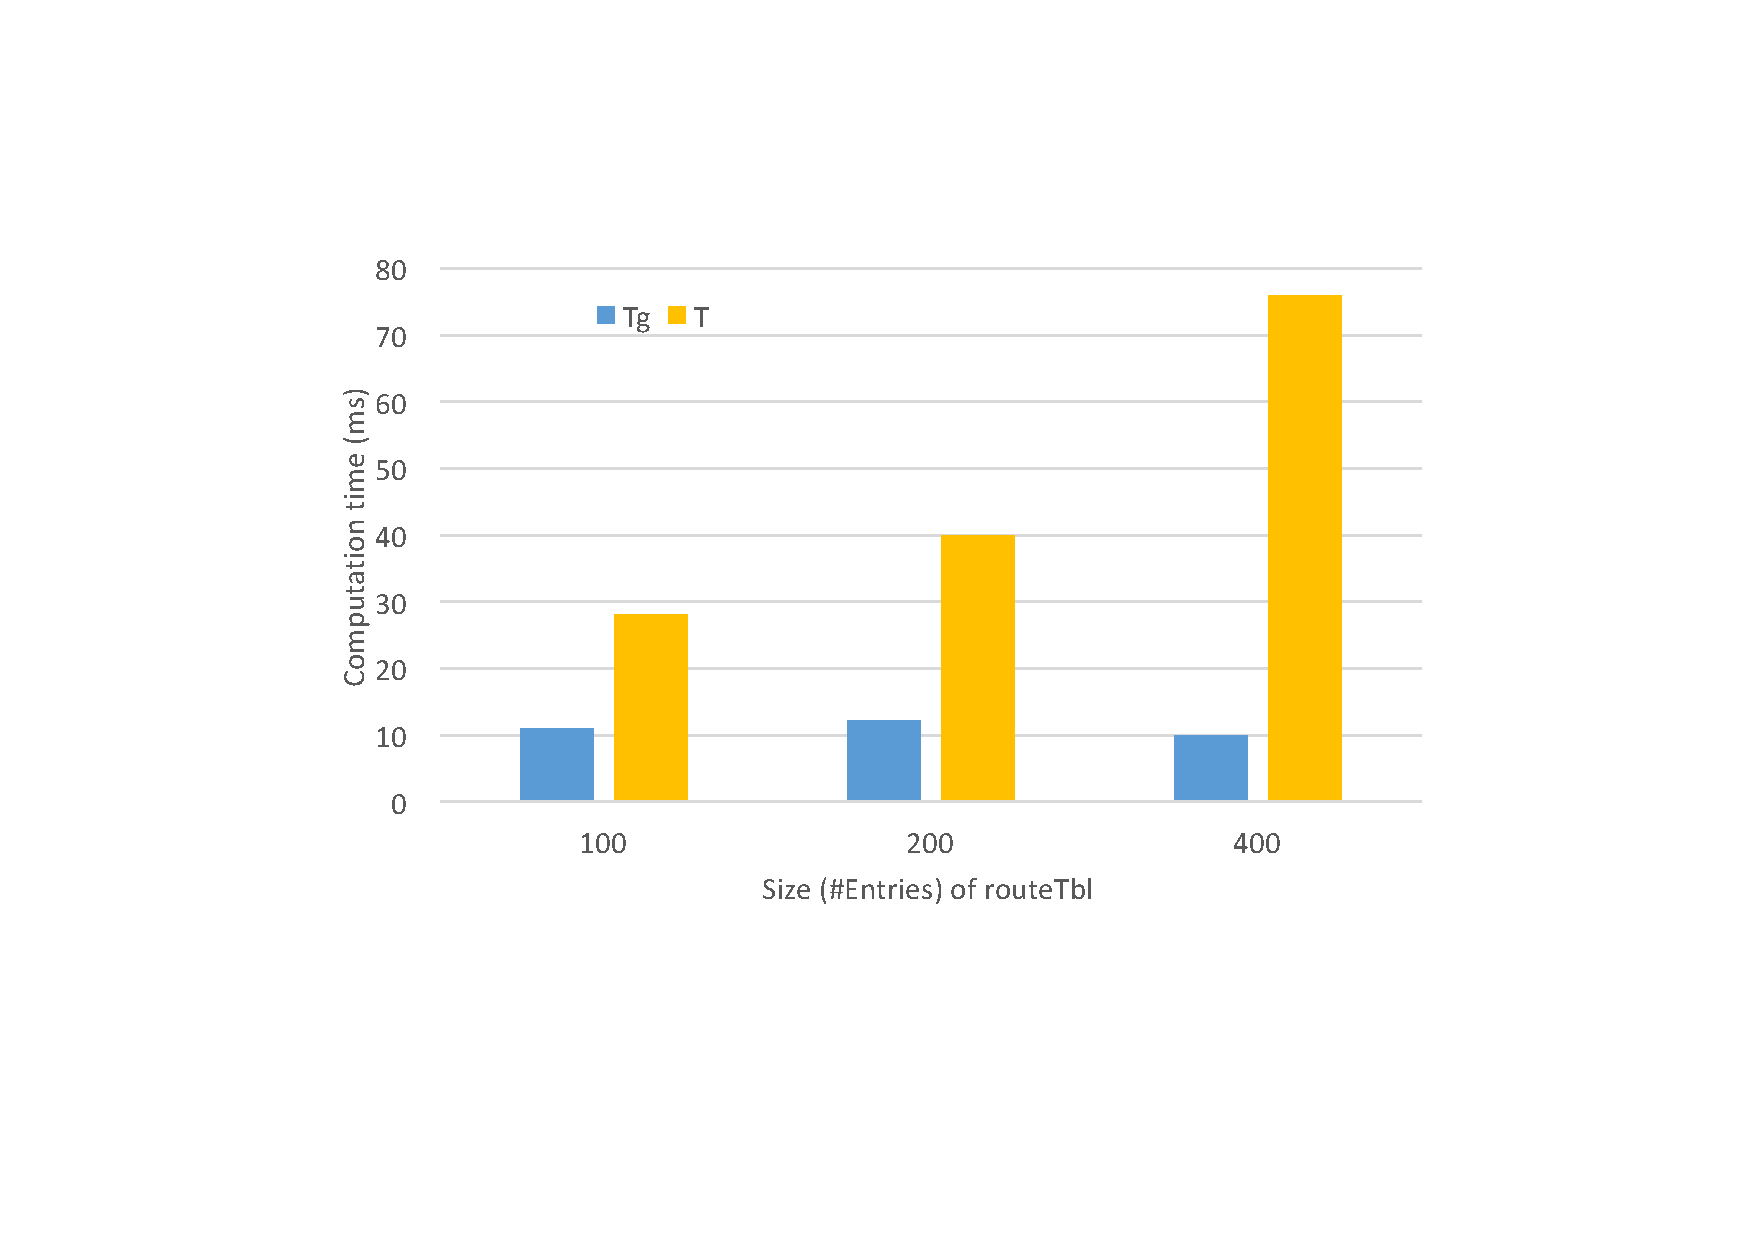
\includegraphics[width=0.4\textwidth]{figures/figure-eval-t2.pdf}}
  % \caption{计算$\tau(\texttt{simpleRoute})$和$\tau_G(\texttt{simpleRoute})$的所需时间。}

  \begin{subfigure}[b]{0.4\textwidth}
      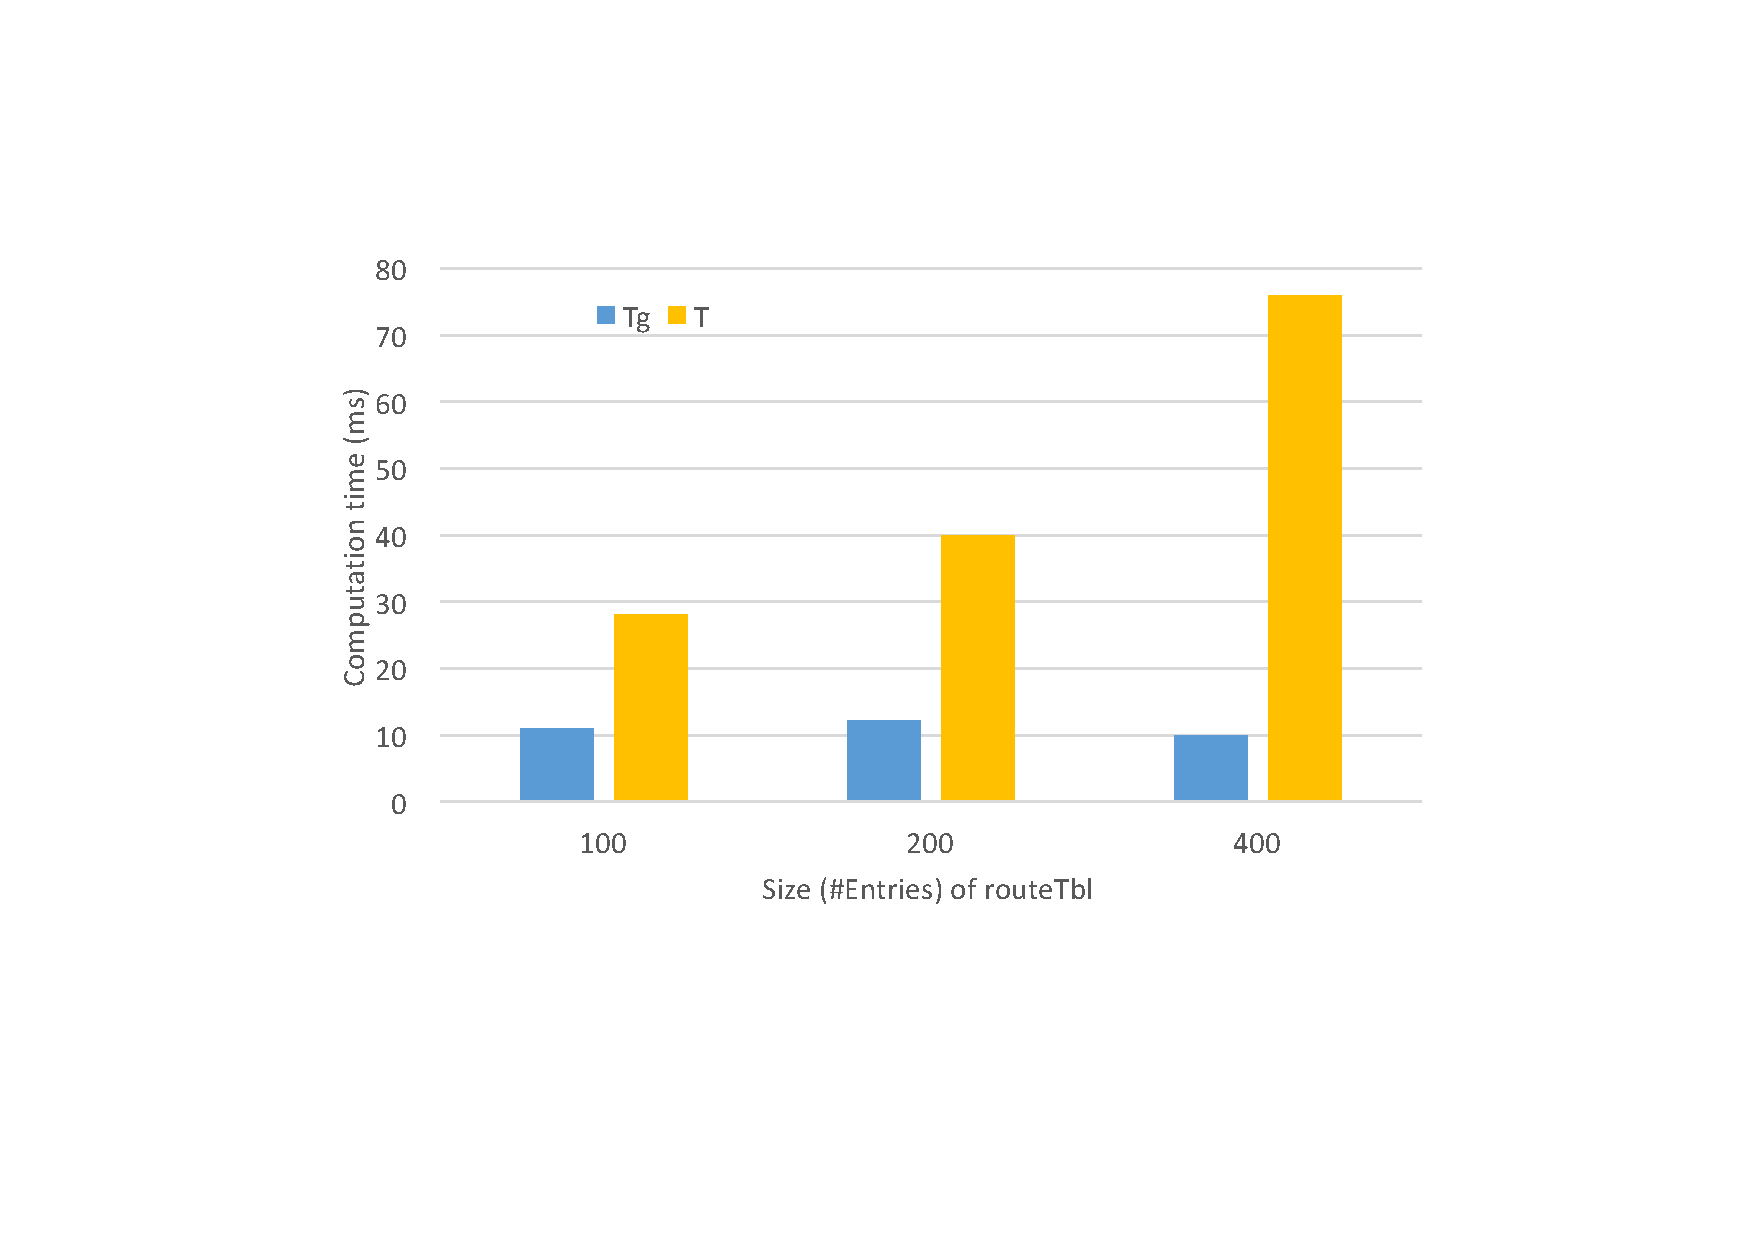
\includegraphics[width=\textwidth]{figures/figure-eval-t2.pdf}
      \caption{表大小变化}  %% TODO fix position 计算$\tau(\texttt{simpleRoute})$和$\tau_G(\texttt{simpleRoute})$的所需时间。
      \label{cap:fig:eval-ct:b}
  \end{subfigure}
  \caption{评估结果}  % TODO: 标题
  \label{cap:fig:eval-ct}
\end{figure}




\subsection{流水线的特征}

我们现在评估流水线特征的计算时间和压缩性。其中压缩性表示特征函数的输出所占存储大小与$M$的全部可能所占存储大小的比值。我们考虑以下流水线进行评估:

%We have examined the characterization of a pipeline by evaluating the computation time and compactness of characterization functions of several pipelines. The compactness of a characterization function of a pipeline represents the output memory utilization of the characterization function compared with the size of all the possible $M$. We use the following pipelines in the evaluation:

\begin{enumerate}
  \item \textbf{OF-DPA Abstract Switch 2.0}: OpenFlow抽象数据平面抽象交换机2.0(OF-DPA)是基于OpenFlow 1.3.4协议的抽象交换机模型,并在OpenFlow协议下允许对基于Broadcom的交换机进行编程。我们考虑了两个OF-DPA流表配置:(1)桥接和路由(BR);(2)数据中心覆盖隧道(OT),它们分别有5个阶段(7个流表)和3个阶段(3个表)。\cite{OF-DPA}

  \item \textbf{PicOS}: PicOS是一个应用于白盒交换机的网络操作系统。它提供了跨HP、Edgecore和Pica交换机的可编程性。我们考虑PicOS提供的两个固定流水线:(1)IP路由流水线(IPR);(2)策略路由流水线(PR),分别包含4个和5个表对应在4和5个阶段。\cite{PicOS}
\end{enumerate}

\para{结果}:表\ref{cap:tbl:table3}是我们对评估流水线的特征结果。其中,我们说在一个流水线$pl$中$M$有效,所指的是$\kappa_\rho(\rho)(M)$的值可以通过$\kappa_\rho(\rho)(M)$定义的第一个公式算出。结果表明,尽管在理论上$\mathcal{M}$子集的数量巨大,但实际上有效$M$并不多。同时流水线特征的计算也非常小。


%shows the characterization results of several pipelines including four real pipeline structures and the example pipeline, \exampledp. We say a set of packet match fields $M$ is valid in a pipeline $p$ means the value of $\kappa_\rho(\rho)(M)$ can be computed by the first formula in the definition of $\kappa_\rho(\rho)(M)$.  The result shows that though there are many combinations of $M$ for the output of characterization of a pipeline, the real memory utilization should be small. Also, it shows the computation of pipeline characterization is very fast.

\begin{table}[t]
\centering
\scalebox{0.8}{
\begin{tabular}{ | l | l | l | l | l | }
    \hline
    流水线 & \#路径数量 & 时间 (ms) & \#有效 $M$ & \#$M$ \\
    \hline
    \exampledp & 3 & 8 & 6 & 22 \\
    PicOS BR & 4 & 13 & 19 & $3*(2^{24})+2^7$ \\
    PicOS OT & 2 & 7 & 5 & $2^{24} + 16$ \\
    Broadcom IPR & 1 & 7 & 4 & $2^7$ \\
    Broadcom PR & 3 & 9 & 14 & $2*(2^{24})+2^7$ \\
    \hline
  \end{tabular}
  }

\vspace{2mm}
\caption{流水线的特征结果。}
\label{cap:tbl:table3}
\end{table}



\subsection{流水线实现的分析}

我们现在评估在流水线中成功实现函数的百分比,以查看成功实现的因素。我们考虑具有不同表内容的示例函数\texttt{onPkt}。具体来说,对于\texttt{condTbl}和\texttt{hostTbl},我们随机设置表的输出值,范围从10到30。这意味着\texttt{dstCond}和\texttt{dstSW}的域大小是从10到30(即平均域大小为20)。对于流水线方面,我们随机决定表的数量(从2到4)以及每个表的输出寄存器的位长(从4到10)。另外我们设置生成的流水线的匹配字段必须包含\texttt{onPkt}所需的五个匹配字段,并且每个匹配字段只能出现在一个表中。最后我们通过实现定理计算\texttt{onPkt}的成功实现百分比和生成的流水线。


%We now evaluate the percentage of successful realization of a function in a pipeline to see the factors of successful realization. We consider the example function \texttt{onPkt} with different content of tables. Specifically, for tables \texttt{condTbl} and \texttt{hostTbl}, we set the number of output values of tables ranging from 10 to 30 randomly, which means the domain size of \texttt{dstCond} and \texttt{dstSW} is from 10 to 30 (\ie, the average domain size is 20). For the pipeline side, we randomly decide the number of tables (from 2 to 4) of a pipeline and the length of bits of registers (from 4 to 10) for each table. Also, we set the match fields of the generated pipeline must contain the five match fields required by \texttt{onPkt} and each match field can only appear in one table. Then, we compute the successful realization percentage of \texttt{onPkt} and the generated pipeline by using the realization theorem.

\begin{figure}  % TODO: fix position
  \centering
  % \subfigure[表数量 = 2]{
  %   \label{cap:fig:eval-rp:a} %% label for first subfigure
  %   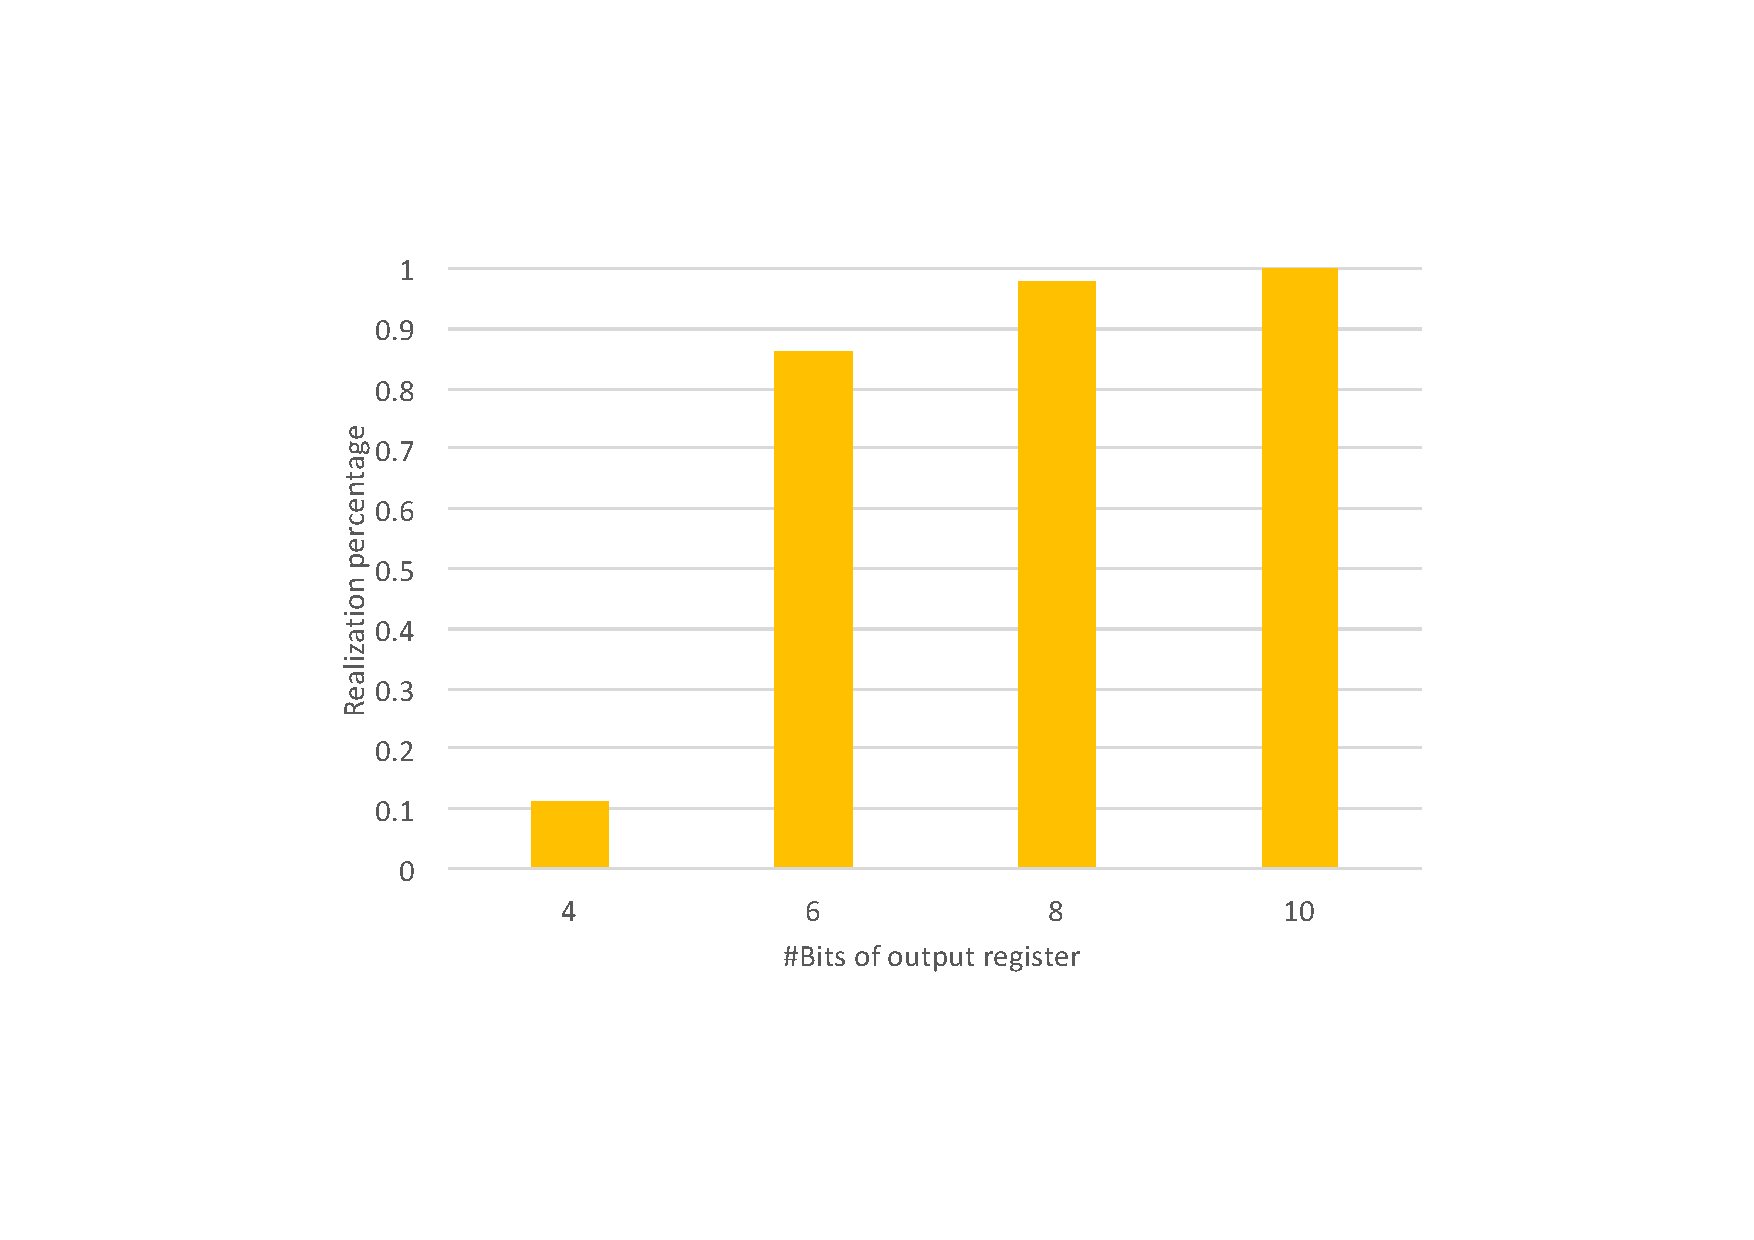
\includegraphics[width=0.4\textwidth]{figures/figure-eval-rp-2.pdf}}

  \begin{subfigure}[b]{0.4\textwidth}
      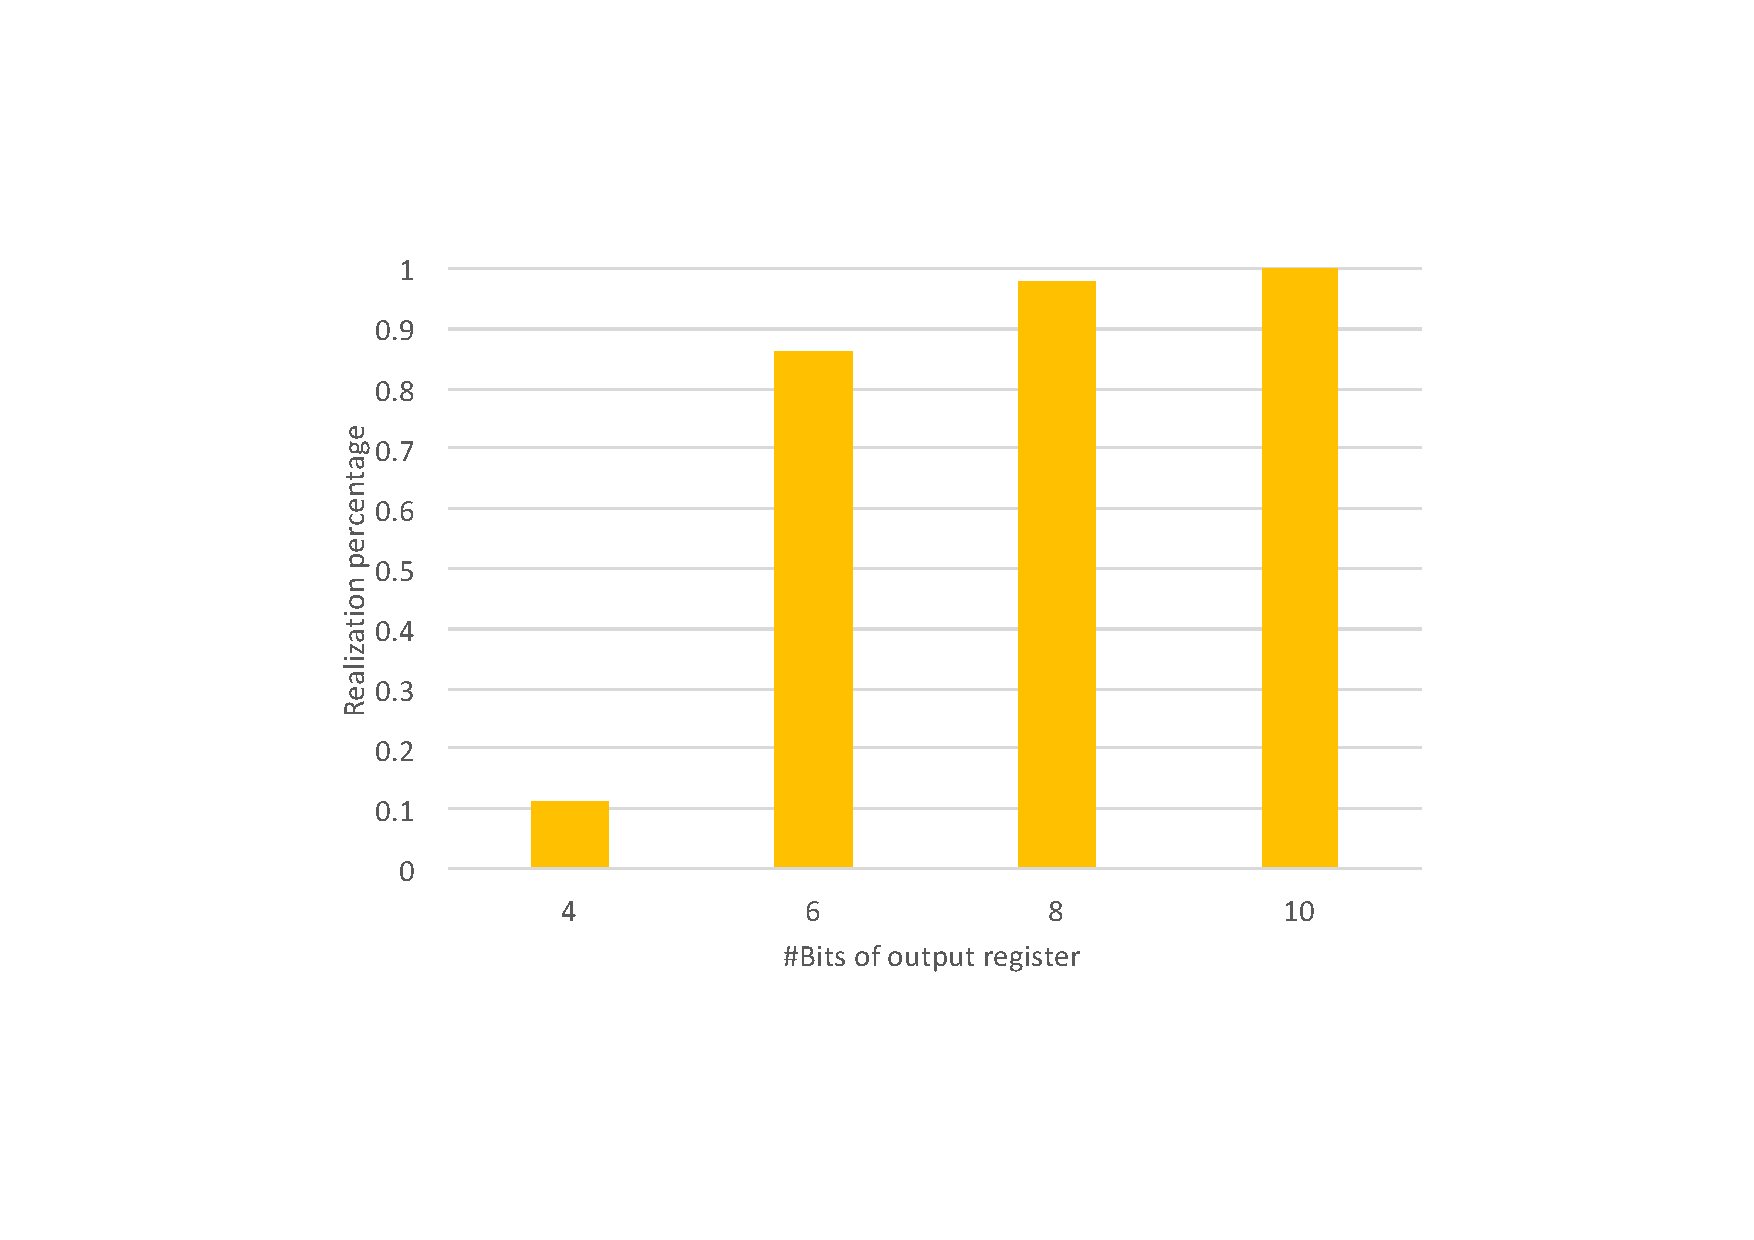
\includegraphics[width=\textwidth]{figures/figure-eval-rp-2.pdf}
      \caption{表数量 = 2}
      \label{cap:fig:eval-rp:a}
  \end{subfigure}

  \hspace{1in}
  % \subfigure[表数量 = 3]{
  %   \label{cap:fig:eval-rp:b} %% label for second subfigure
  %   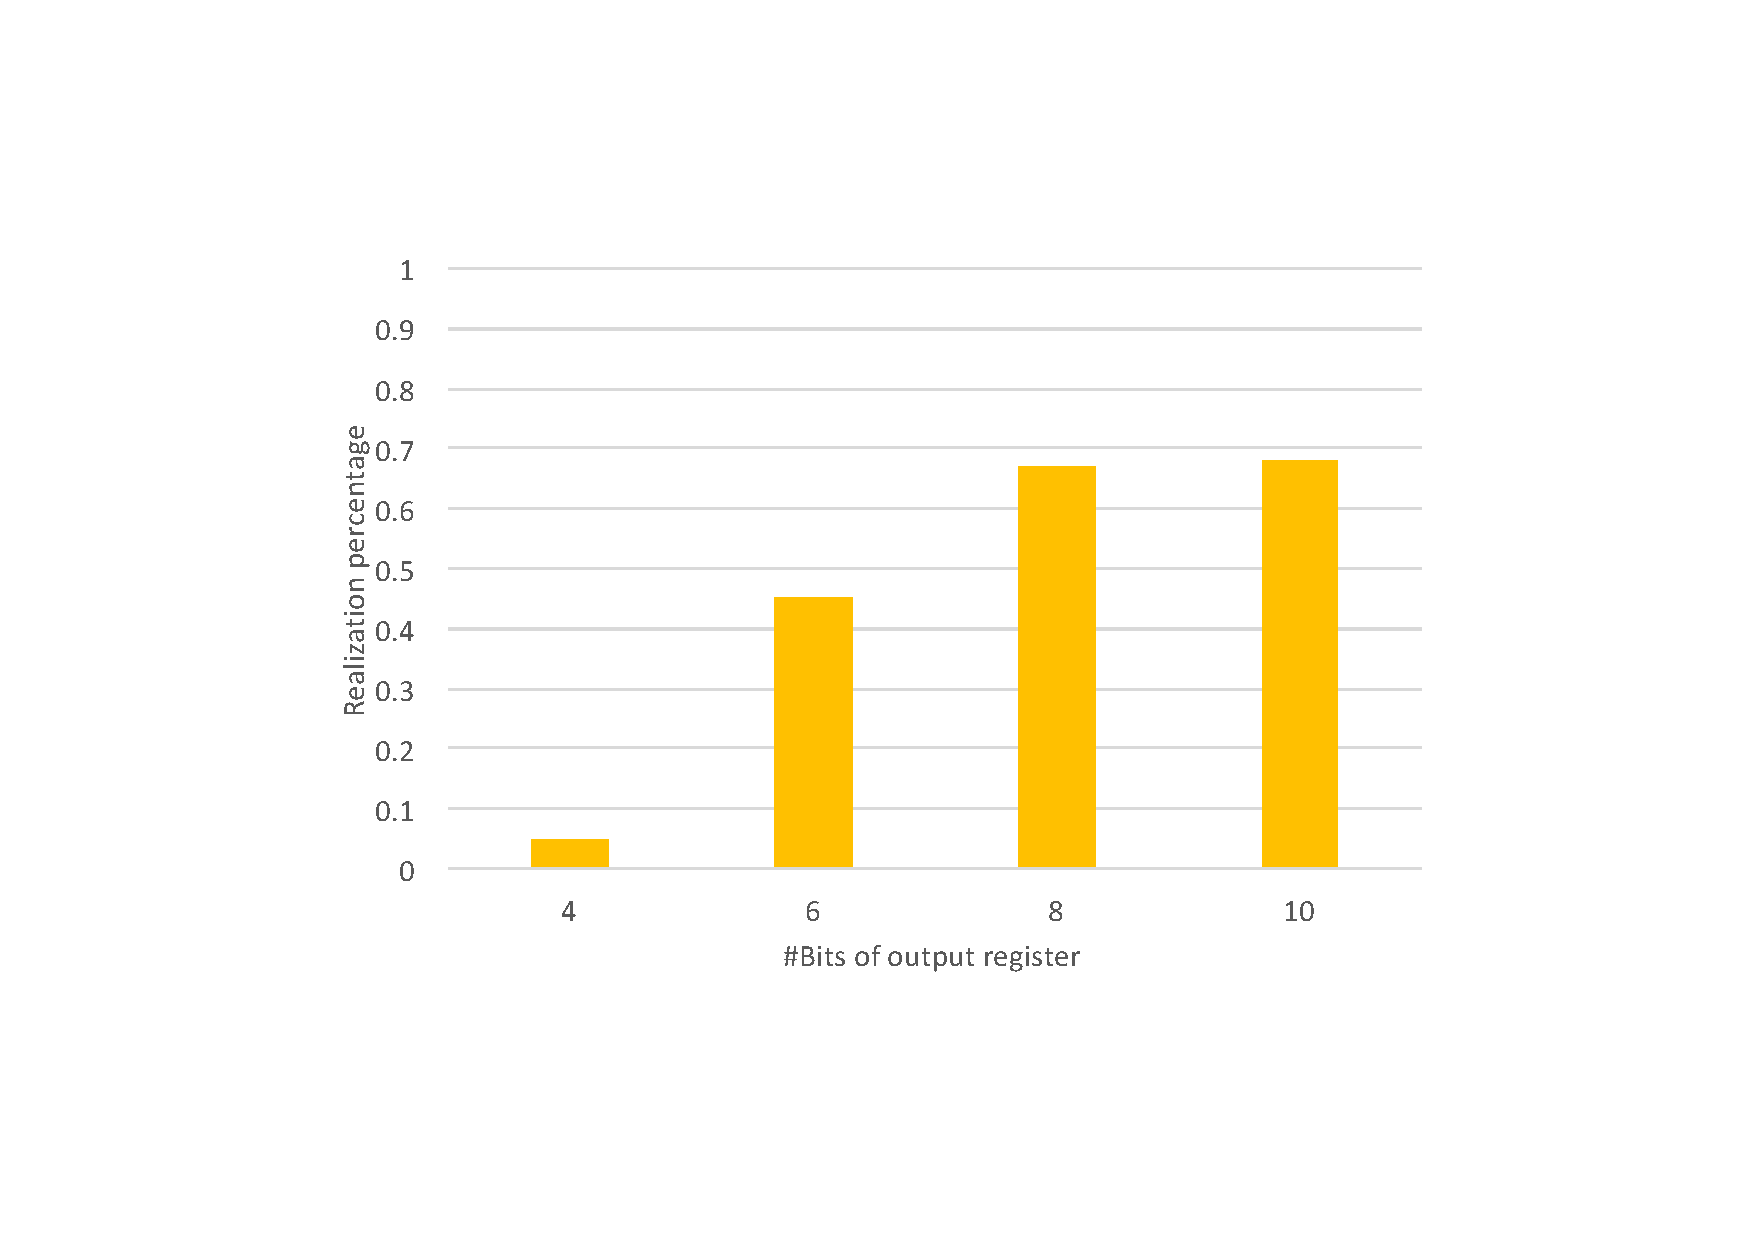
\includegraphics[width=0.4\textwidth]{figures/figure-eval-rp-3.pdf}}

  \begin{subfigure}[b]{0.4\textwidth}
      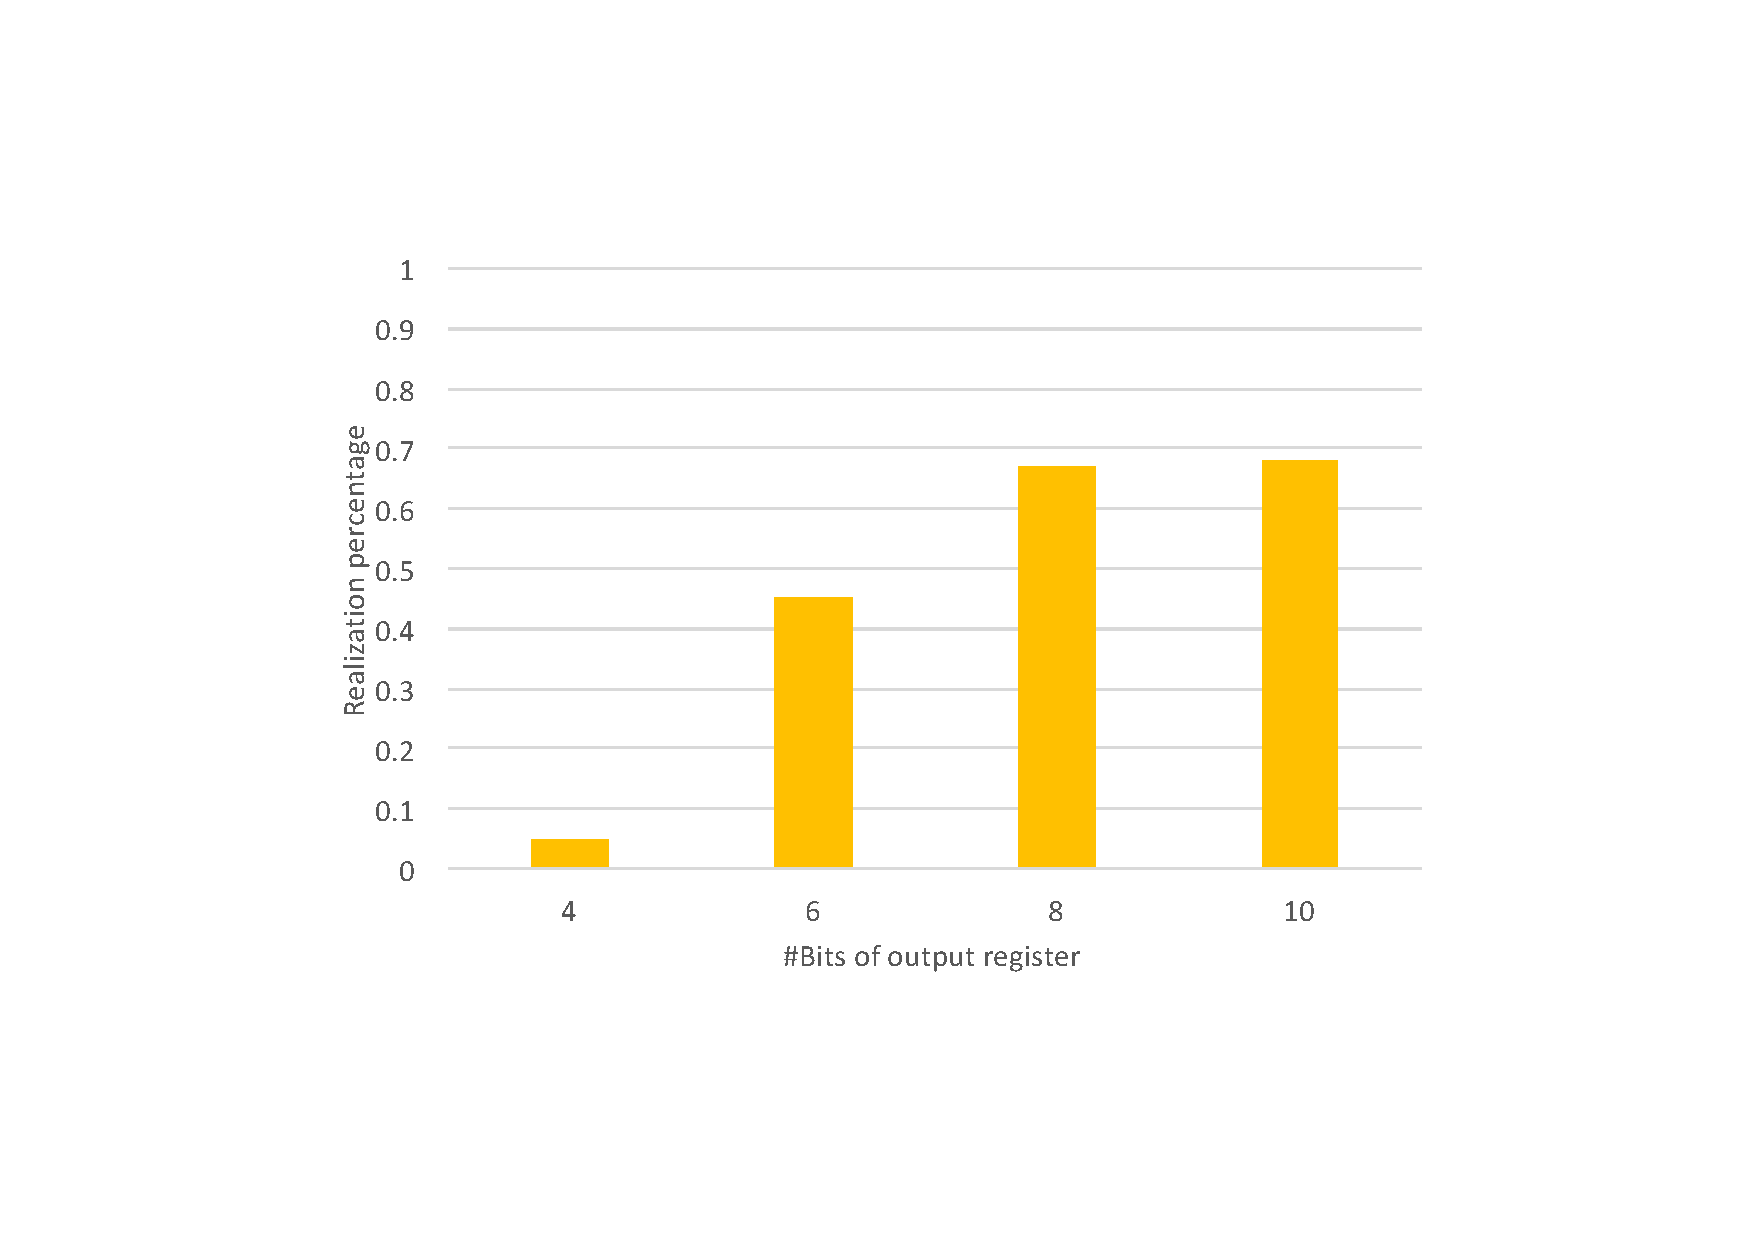
\includegraphics[width=\textwidth]{figures/figure-eval-rp-3.pdf}
      \caption{表数量 = 3}
      \label{cap:fig:eval-rp:b}
  \end{subfigure}

  % \subfigure[表数量 = 4]{
  %   \label{cap:fig:eval-rp:c} %% label for second subfigure
  %   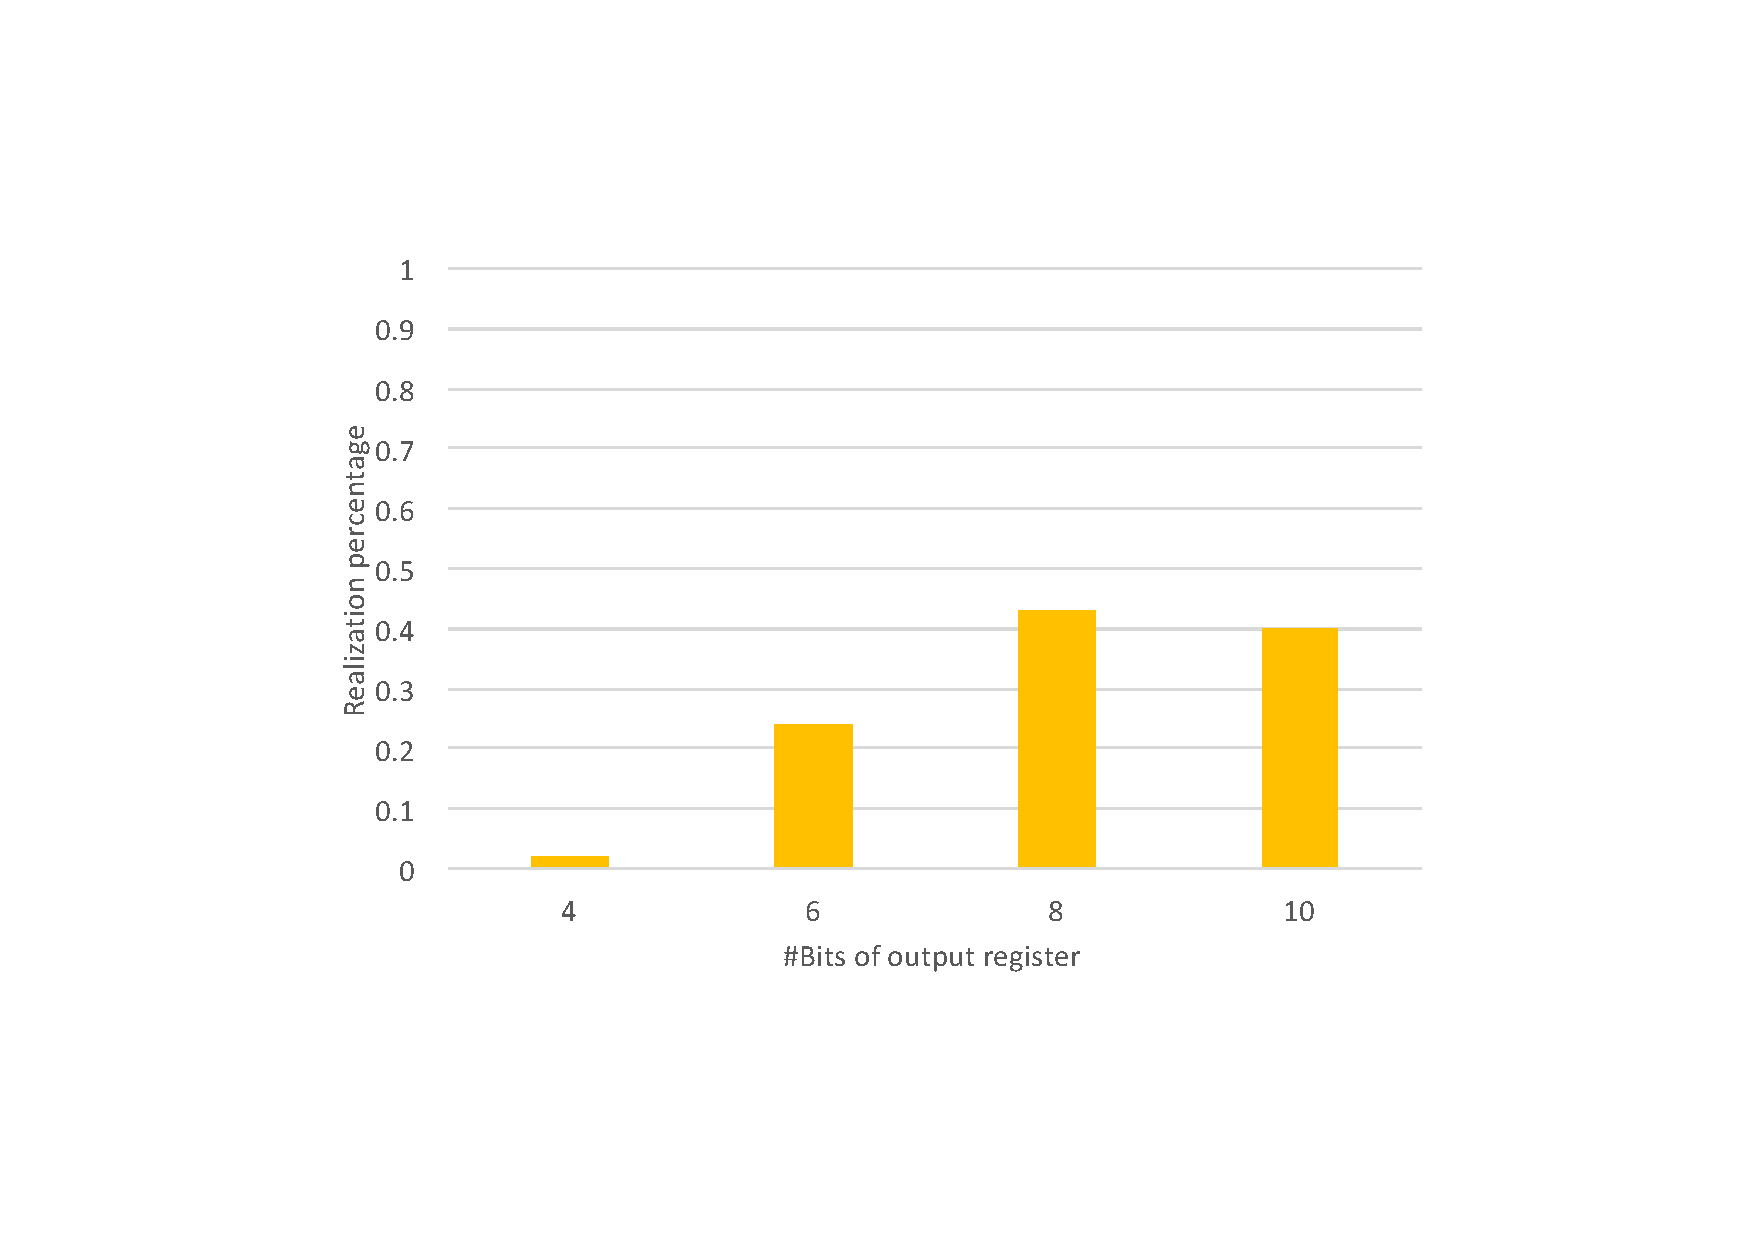
\includegraphics[width=0.4\textwidth]{figures/figure-eval-rp-4.pdf}}

  \begin{subfigure}[b]{0.4\textwidth}
      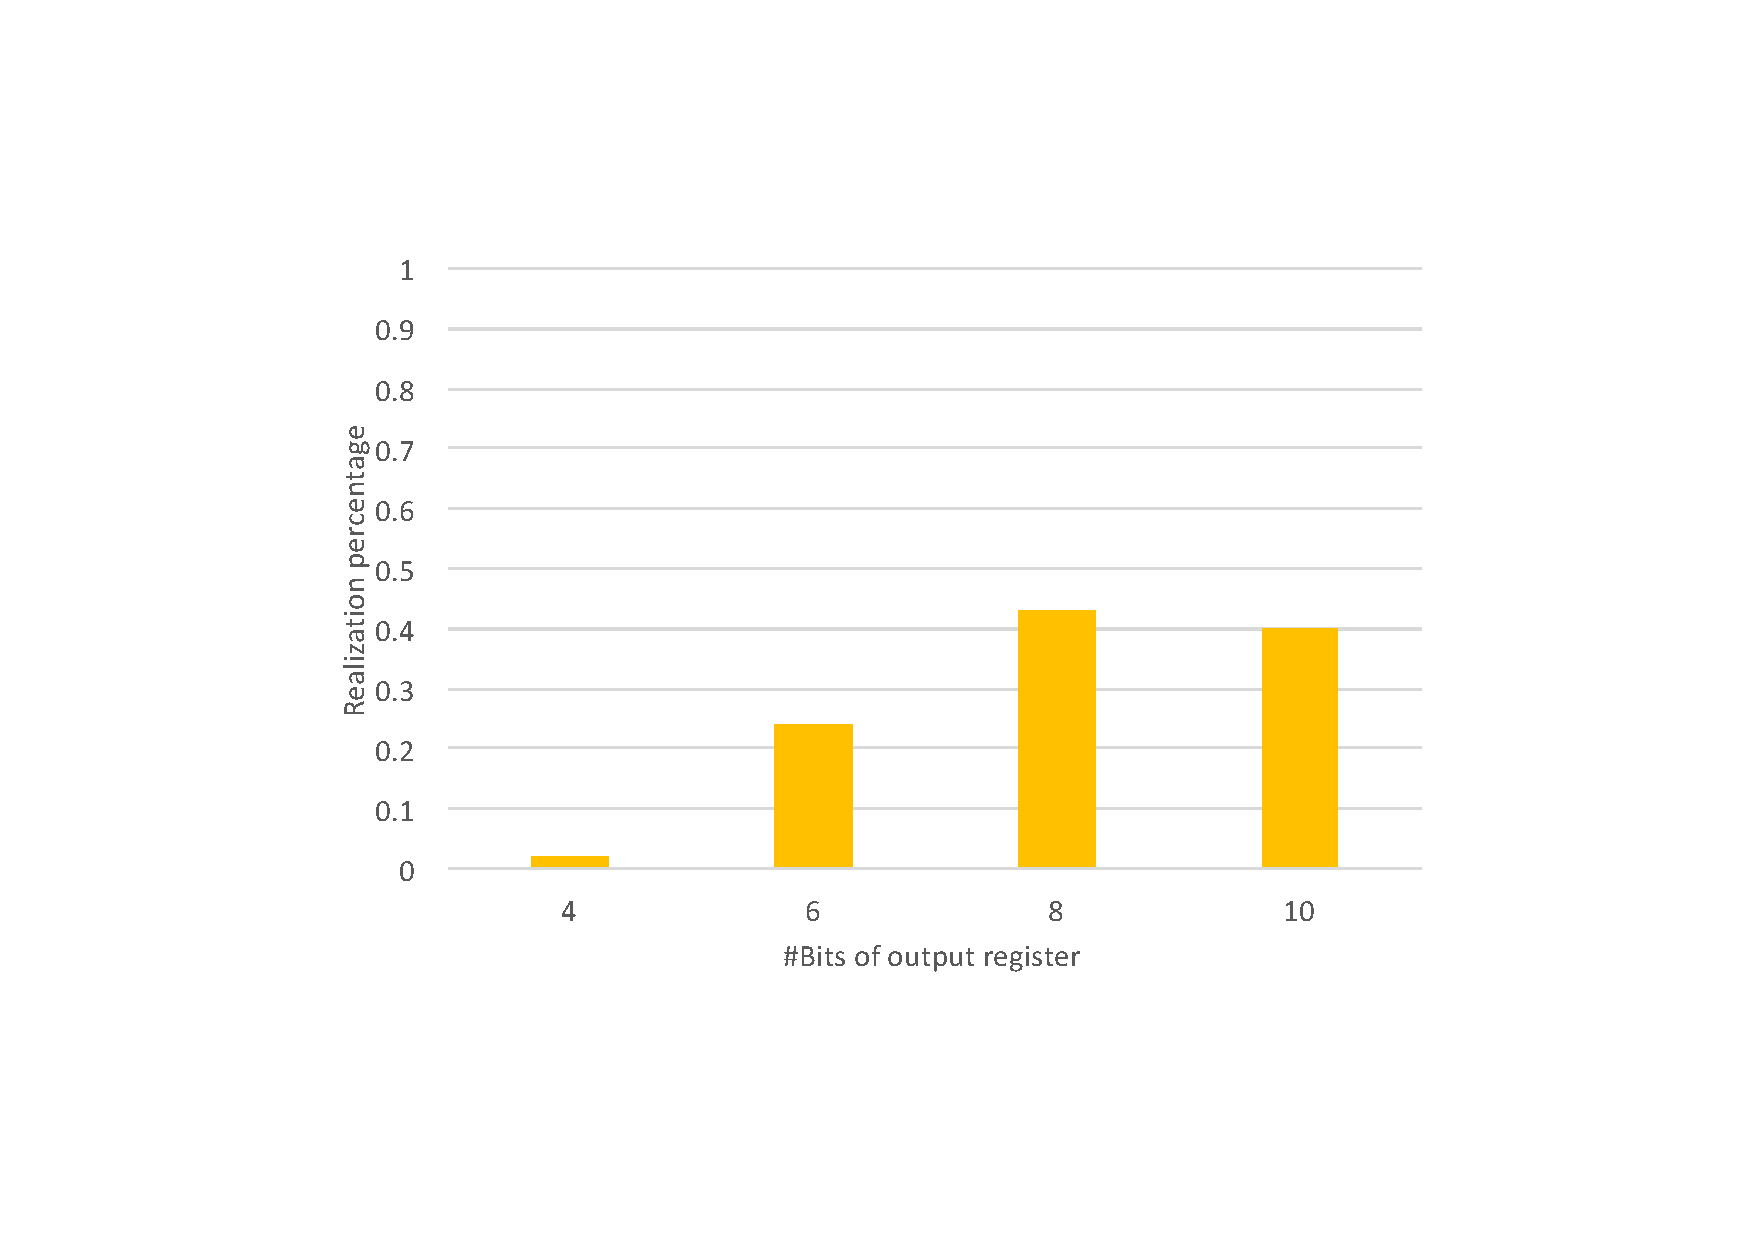
\includegraphics[width=\textwidth]{figures/figure-eval-rp-4.pdf}
      \caption{表数量 = 4}
      \label{cap:fig:eval-rp:c}
  \end{subfigure}

  \caption{对于不同表数量和寄存器位长度的实现成功百分比。}
  \label{cap:fig:eval-rp} %% label for entire figure
\end{figure}

\para{结果}:如图~\ref{cap:fig:eval-rp}所示。
其中,图\ref{cap:fig:eval-rp:a}考虑的具有两个表的流水线;图\ref{cap:fig:eval-rp:b}为3个表的流水线;图\ref{cap:fig:eval-rp:c}为4个表。
对于每种情况,我们变化每个表的寄存器位长度,并计算实现成功的百分比。
从图~\ref{cap:fig:eval-rp:a}的结果中,我们可以发现具有更多位寄存器的流水线可以实现更高百分比的功能。
但是,当长度大于一定阈值时,成功实现百分比不会增加太多。阈值由函数中变量域的大小确定。
如图\ref{cap:fig:eval-rp:a}所示,实现成功的百分比在4位和6位寄存器长度之间的差距(即等效类的可用大小从16到64)可以通过变量的平均域大小(即20)在16到64之间的范围来解释。



%The result is shown in Fig.~\ref{fig:eval-rp}. Specifically, Fig.~\ref{fig:eval-rp:a} considers the pipeline with 2 tables; Fig.~\ref{fig:eval-rp:b} considers the pipeline with 3 tables; Fig.~\ref{fig:eval-rp:c} considers the pipeline with 4 tables. For each case, we compute the successful realization percentage with different length of bits of registers for each table. From the result of Fig.~\ref{fig:eval-rp:a}, we can find that a pipeline with more bits of registers can realize a function in a higher percentage. However, when the length is larger than a threshold, the successful realization percentage does not increase much. The threshold is determined by the size of domain of variables in the function. As shown in Fig.~\ref{fig:eval-rp:a}, the gap of successful realization percentage between 4 bits and 6 bits of length of registers (\ie, the available size of equivalent classes from 16 to 64) can be explained by the fact that the average domain size of variables (\ie, 20) is in the range between 16 and 64.

进一步,我们可以发现流水线的结构也决定了实现成功的百分比。具有2个表的流水线(即没有分支)具有相对较高的成功实现百分比,而具有3或4个可能包含分支的表的流水线具有较低的实现百分比,因为这些流水线的结构可能并不好(即匹配字段和表之间的随机映射)。


%Furthermore, we can find the structure of pipelines also determines the realization percentage. A pipeline with 2 tables (\ie, there is no branch in the pipeline) has a relatively high successful realization percentage, while a pipeline with 3 or 4 tables which may contain branches has a low realization percentage as the structure of the pipeline is not well organized (\ie, the random mapping between matches fields and tables).

\section{本章小结}

本章我们针对高级SDN程序对于固定结构数据通路的实现问题,提出了将高级 SDN 程序和底层数据通路统一的特征空间。并将实现问题转化为空间中的比较问题,并给出流水线实现定理以及相关证明。实验表明,虽然我们的流水线实现定理给出的是充分条件,但其严密性较好,在实际情况中不会太大误差。




\printbibliography[heading=bibintoc]

\end{document}